% Sablon pentru realizarea lucrarii de licenta, conform cu recomandarile
% din ghidul de redactare:
% - https://fmi.unibuc.ro/finalizare-studii/
% - https://drive.google.com/file/d/1xj9kZZgTkcKMJkMLRuoYRgLQ1O8CX0mv/view

% Multumiri lui Gabriel Majeri, acest sablon a fost creat pe baza
% codului sursa a lucrarii sale de licenta. 
% Codul sursa: https://github.com/GabrielMajeri/bachelors-thesis
% Website: https://www.gabrielmajeri.ro/
%
% Aceast sablon este licentiat sub Creative Commons Attribution 4.0 International License.

\documentclass[12pt, a4paper]{report}

\setcounter{secnumdepth}{3}
\setcounter{tocdepth}{3}

% Suport pentru diacritice și alte simboluri
\usepackage{fontspec}
\usepackage{multicol}
\usepackage{booktabs}
% Suport pentru mai multe limbi
\usepackage{polyglossia}

% Setează limba textului la română
\setdefaultlanguage{romanian}
% Am nevoie de engleză pentru rezumat
\setotherlanguages{english}

% Indentează și primul paragraf al fiecărei noi secțiuni
\SetLanguageKeys{romanian}{indentfirst=true}

% Suport pentru diferite stiluri de ghilimele
\usepackage{csquotes}
\usepackage{float}
\usepackage{subcaption}
\usepackage{caption}
\usepackage{chngcntr}

\floatstyle{plain}
\newfloat{lstro}{htbp}{lop}
\floatname{lstro}{Lista}           
\counterwithin{lstro}{chapter}   

\DeclareQuoteStyle{romanian}
  {\quotedblbase}
  {\textquotedblright}
  {\guillemotleft}
  {\guillemotright}

% Utilizează biblatex pentru referințe bibliografice
\usepackage[
    maxbibnames=50,
    sorting=nty
]{biblatex}

\addbibresource{bibliography.bib}

% Setează spațiere inter-linie la 1.5
\usepackage{setspace}
\onehalfspacing

% Modificarea geometriei paginii
\usepackage{geometry}

% Include funcțiile de grafică
\usepackage{graphicx}
% Încarcă imaginile din directorul `images`
\graphicspath{{./images/}}

% Listări de cod
\usepackage{listings}
\usepackage{xcolor}
\definecolor{LightGray}{gray}{0.9}

\usepackage{minted}

% Linkuri interactive în PDF
\usepackage[
    colorlinks,
    linkcolor={blue},
    menucolor={blue},
    citecolor={blue},
    urlcolor={blue}
]{hyperref}

% Simboluri matematice codificate Unicode
\usepackage[warnings-off={mathtools-colon,mathtools-overbracket}]{unicode-math}

% Comenzi matematice
\usepackage{amsmath}
\usepackage{mathtools}

% Formule matematice
\newcommand{\bigO}[1]{\symcal{O}\left(#1\right)}
\DeclarePairedDelimiter\abs{\lvert}{\rvert}

% Suport pentru rezumat în două limbi
% Bazat pe https://tex.stackexchange.com/a/70818
\newenvironment{abstractpage}
  {\cleardoublepage\vspace*{\fill}\thispagestyle{empty}}
  {\vfill\cleardoublepage}
\renewenvironment{abstract}[1]
  {\bigskip\selectlanguage{#1}%
   \begin{center}\bfseries\abstractname\end{center}}
  {\par\bigskip}

% Suport pentru anexe
\usepackage{appendix}
\renewcommand{\appendixpagename}{Anexe}
\renewcommand{\appendixname}{Anexă}
% Stiluri diferite de headere și footere
\usepackage{fancyhdr}

% Metadate
\title{Un pas spre înțelegerea alfabetului ASL}
\author{Stratulat Vladimir}

% Generează variabilele cu @
\makeatletter

\begin{document}

% Front matter
\cleardoublepage
\let\ps@plain

% Pagina de titlu
\begin{titlepage}

% Redu marginile
\newgeometry{left=2cm,right=2cm,bottom=1cm}

\begin{figure}[!htb]
    \centering
    \begin{minipage}{0.2\textwidth}
        
\includegraphics[width=\linewidth]{images/0-title/logo-ub.png}
    \end{minipage}
    \begin{minipage}{0.5\textwidth}
        \large
        \vspace{0.2cm}
        \begin{center}
            \textbf{UNIVERSITATEA DIN BUCUREȘTI}
        \end{center}
        \vspace{0.3cm}
        \begin{center}
            \textbf{
                FACULTATEA DE \\
                MATEMATICĂ ȘI INFORMATICĂ
            }
        \end{center}
    \end{minipage}
    \begin{minipage}{0.2\textwidth}
        
\includegraphics[width=\linewidth]{images/0-title/logo-fmi.png}
    \end{minipage}
\end{figure}

\begin{center}
\textbf{SPECIALIZAREA INFORMATICĂ}
\end{center}

\vspace{1cm}

\begin{center}
\Large \textbf{Lucrare de licență}
\end{center}

\begin{center}
\huge \textbf{\MakeUppercase{\@title}}
\end{center}

\vspace{3cm}

\begin{center}
\large \textbf{Absolvent \\ \@author}
\end{center}

\vspace{0.25cm}

\begin{center}
\large \textbf{Coordonator științific \\ Conf. Dr. Alexe Bogdan}
\end{center}

\vspace{2cm}

\begin{center}
\Large \textbf{București, iunie 2025}
\end{center}
\end{titlepage}
\restoregeometry
\newgeometry{
    margin=2.5cm
}

\fancypagestyle{main}{
  \fancyhf{}
  \renewcommand\headrulewidth{0pt}
  \fancyhead[C]{}
  \fancyfoot[C]{\thepage}
}



% Rezumatul
\begin{abstractpage}

\begin{abstract}{romanian}

Scopul acestei lucrări este facilitarea interacțiunii cu persoanele care prezintă deficiențe de auz și/sau vorbire prin eliminarea barierei de comunicare prezente între acestea și indivizii din populația generală.

Soluția propusă constă într-o aplicație mobilă capabilă să detecteze și să traducă semnele alfabetului \textit{American Sign Language} (ASL). Nucleul aplicației este reprezentat de o rețea neuronală convoluțională, integrată într-o aplicație dezvoltată pentru sistemul de operare Android. Modelul urmează o arhitectură proprie, inspirată din modele performante existente, și este antrenat pe un set de date construit din multiple surse. 

În procesul de antrenare au fost utilizate tehnici moderne de regularizare, precum \textit{dropout}, \textit{label smoothing} și augmentarea datelor, cu scopul îmbunătățirii generalizării modelului. Acuratețea finală pe un set de testare reprezentativ pentru mediul real este de peste $91\%$.

Se poate concluziona că lucrarea și-a atins obiectivul, modelul propus fiind performant și eficient, iar aplicația oferă o bază pentru extinderea cercetării către recunoașterea cuvintelor și a propozițiilor.
 
\end{abstract}

\begin{abstract}{english}

The aim of this thesis is to bridge the gap between individuals with hearing and/or speech impairments and the general population.

The proposed solution consists of a mobile application capable of detecting and translating the American Sign Language (ASL) alphabet. At its core, the application is composed of a convolutional neural network, integrated into an Android mobile application. The model follows a custom architecture, inspired by state-of-the-art models, and was trained on a custom dataset composed of multiple sources.

During the training process, several modern regularization techniques were applied, such as dropout, label smoothing and data augmentation, with the purpose of improving model generalization. The final model achieved an accuracy of over $91\%$ on a test set representative of real-world conditions.

It can be concluded that the thesis reached its goal, the proposed model being accurate and efficient. Moreover, the final application offers a foundation for extending the research towards recognizing words and sentences.

\end{abstract}

\end{abstractpage}
\pagenumbering{gobble}
\tableofcontents
\listoffigures
\listoftables
% Main matter
\cleardoublepage
\pagestyle{main}
\let\ps@plain\ps@main

\pagenumbering{arabic}
\addtocounter{page}{5}
\chapter{Introducere}

Un subdomeniu al inteligenței artificiale care a captat interesul publicului, al sectorului privat și al instituțiilor guvernamentale este vederea artificială. În ultimii ani au fost înregistrate progrese semnificative atât în dezvoltarea de noi metode utilizate în vederea artificială, cât și al capacității de procesare a datelor și implementare a acestor noi algoritmi. Vederea artificială are un rol bine stabilit într-o gamă variată de cazuri, cum ar fi robotica, securitatea unei instituții, industria \textit{software} (recunoaștere facială, realitate augmentată) și, cel mai important pentru lucrarea de față, medicina și accesibilitatea.

Această lucrare își propune să contribuie la apropierea de persoanele care prezintă deficiențe de auz și/sau vorbire. Având în vedere importanța integrării acestora și nevoia de a ușura interacțiunea, vizăm să reducem bariera apărută în comunicare. Aplicația dezvoltată sprijină indivizii care doresc fie să traducă literele exprimate cu ajutorul mâinilor, fie să învețe sau să exerseze alfabetul limbajului american al semnelor (în engl. \textit{American Sign Language} - ASL).

Pentru a ne atinge scopul, utilizăm tehnici de \textit{deep learning} pentru antrenarea unui model bazat pe o rețea neuronală convoluțională (în engl. Convolutional Neural Network - CNN), reprezentând nucleul aplicației mobile Android folosite de utilizator. Aplicația reprezintă interfața prin care utilizatorul interacționează cu rețeaua neuronală antrenată. Aceasta transmite modelului cadrele capturate cu ajutorul camerei dispozitivului, modelul le analizează și returnează rezultatele detecției.

În căutarea unui set de date potrivit pentru antrenare, am observat că majoritatea seturilor de date privind alfabetul ASL conțineau doar imagini similare, fie ca fundal, fie ca poziție a mâinii, făcând dificilă antrenarea unui model asupra unui singur set de date. Pentru a depăși această problemă, s-a optat pentru combinarea mai multor surse, pentru a ajuta modelul în generalizare. Un set de date a fost creat special pentru acest studiu prin înregistrarea video a autorului lucrării și a unui voluntar, trei seturi au fost preluate de pe \textbf{Youtube} \cite{youtube_dataset0, youtube_dataset1, youtube_dataset2}, cinci au fost preluate de pe \textbf{Kaggle} \cite{kaggle_dataset0, kaggle_dataset1, kaggle_dataset2, kaggle_dataset3, kaggle_dataset4}, iar restul de cinci din articole științifice \cite{article_dataset0, article_dataset1, article_dataset2, article_dataset3, article_dataset4}, integrând un total de 14 surse.

Pentru început, am remarcat faptul că seturile de date originale conțineau imagini cu litere aparținând mai multor dialecte ale alfabetului ASL. Prin urmare, materialul oferit de \textit{American Society for Deaf Children} (ASDC), ilustrat în Figura~\ref{fig:exemplu_litere_fingerspell}, servește drept referință în filtrarea manuală a imaginilor.

\begin{figure}[H]
  \centering
  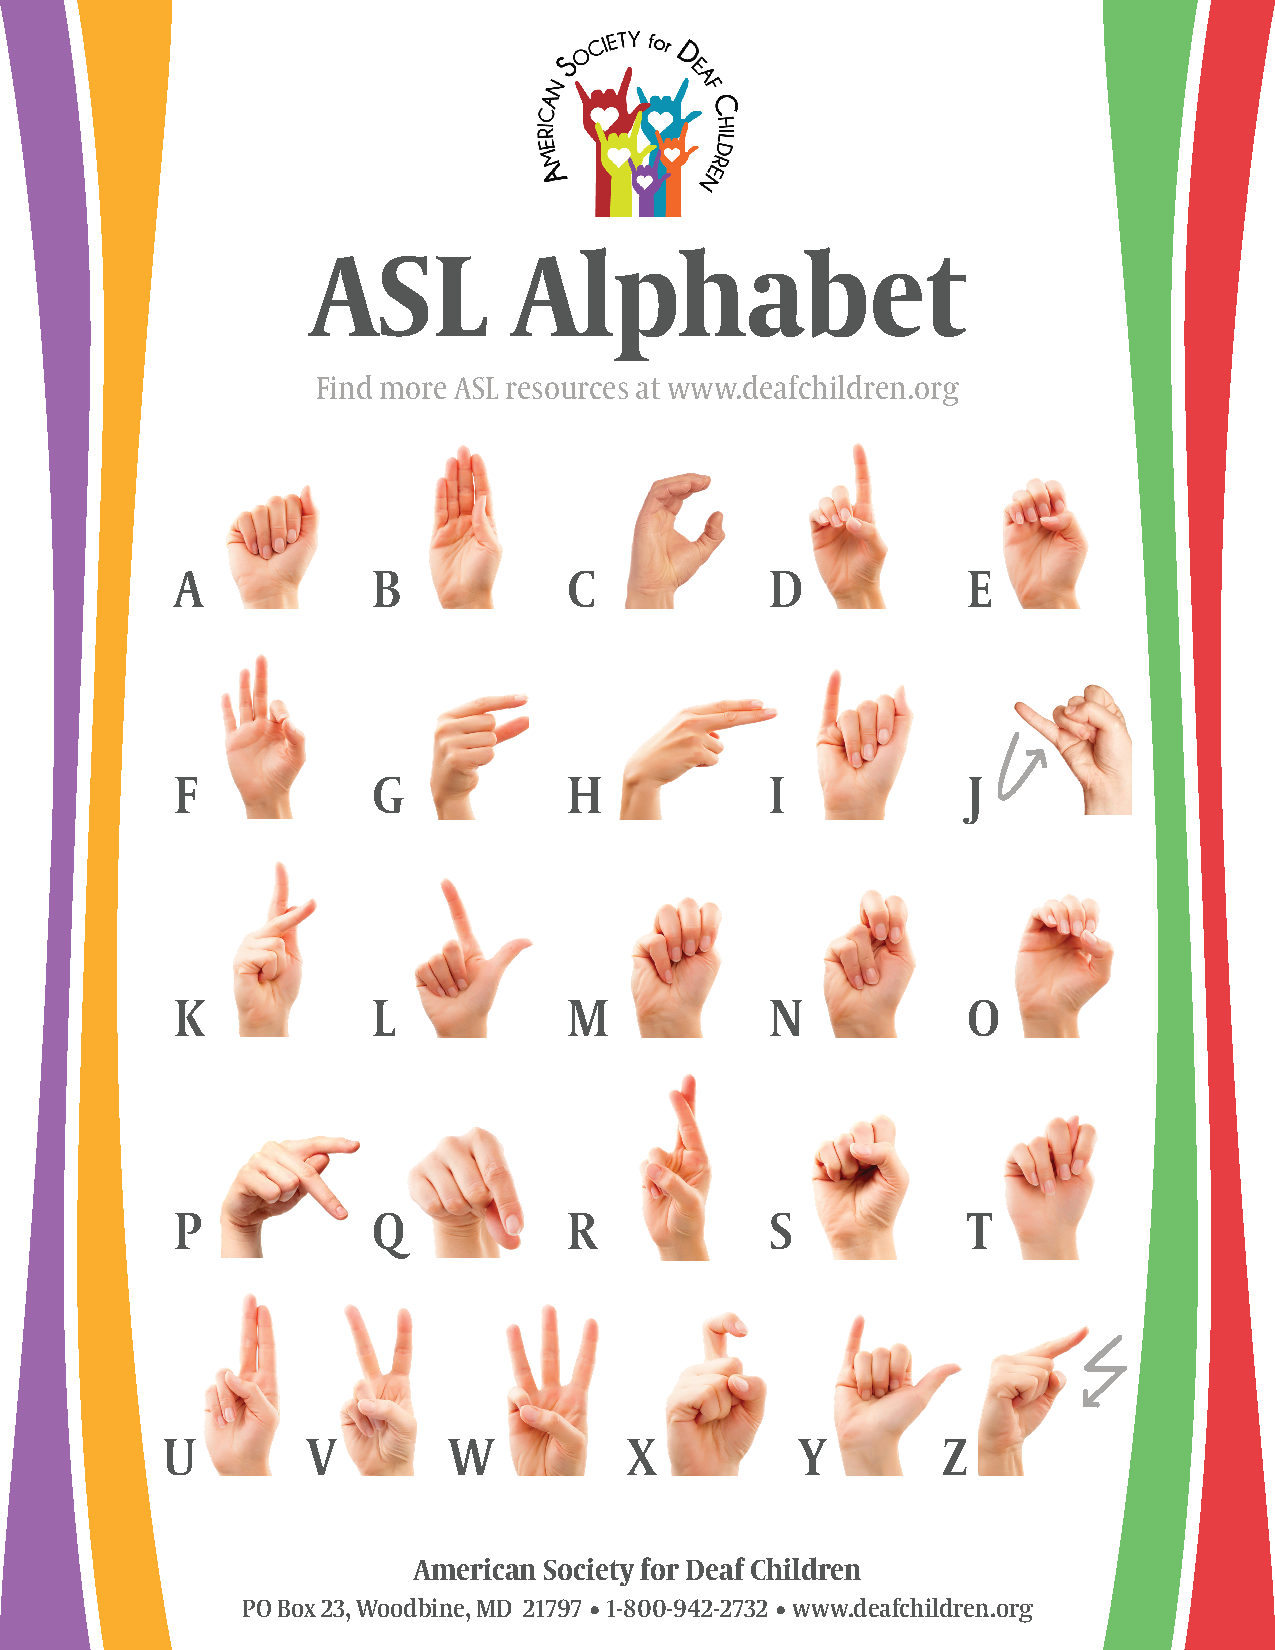
\includegraphics[width=0.5\textwidth]{images/2-recunoasterea-asl/ASL-Alphabet-ASDC.pdf}
  \caption[Alfabetul ASL]{\textbf{Alfabetul ASL}. \textit{Imagine preluată de pe website-ul ASDC \cite{asl_alphabet_chart}. Fiecare palmă reprezintă o literă din alfabet. J și Z presupun mișcare, așadar săgețile indică forma mișcării.}}
  \label{fig:exemplu_litere_fingerspell}
\end{figure}

În cazul în care unul sau mai multe dialecte diferite de cel ilustrat în Figura~\ref{fig:exemplu_litere_fingerspell} aveau reprezentativitate consistentă, s-a decis păstrarea acestora, întrucât modelul este capabil să învețe diferite dialecte pentru o literă, cât timp „vede” destule exemple. Un caz de acest fel poate fi observat în Figura~\ref{fig:p_2_dialecte}.

\begin{figure}[H]
  \centering
  \begin{subfigure}{0.3\textwidth}
    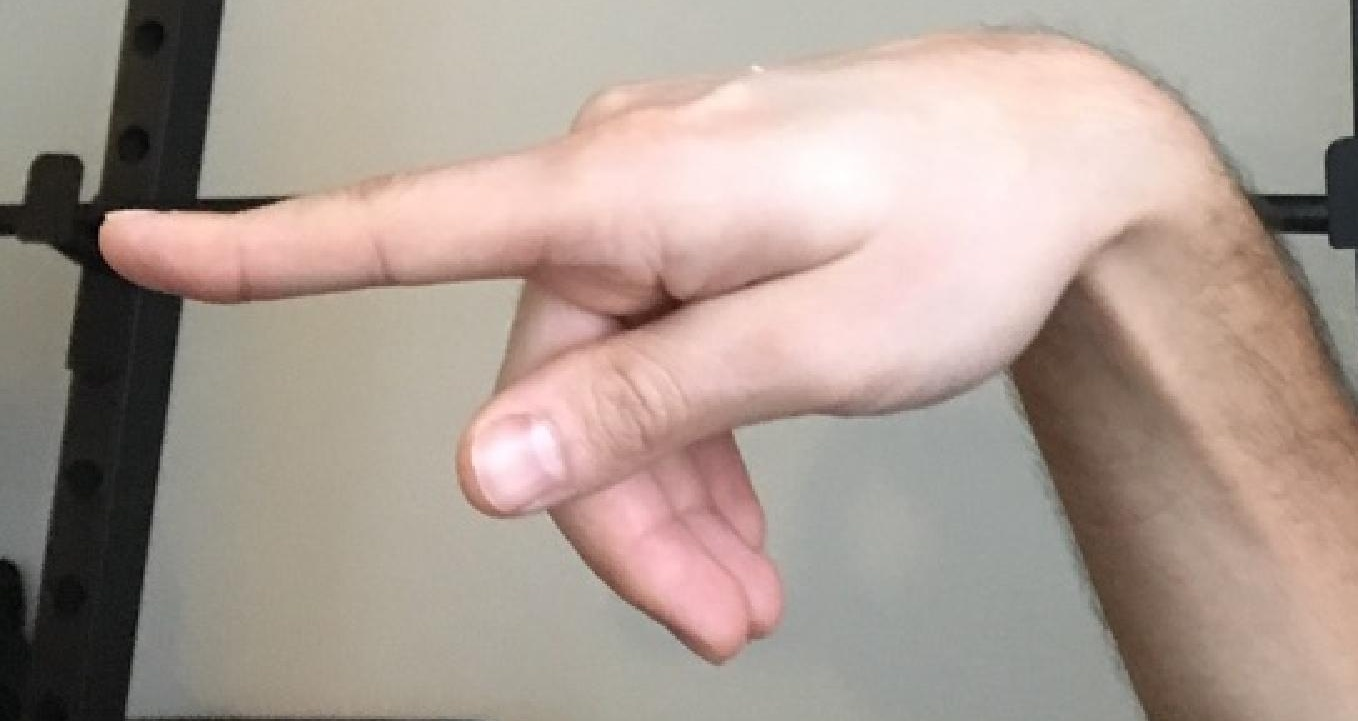
\includegraphics[width=\linewidth]{images/2-recunoasterea-asl/p_dialect1.png}
    \caption{}
    \label{fig:img1}
  \end{subfigure}
    \hspace{0.1\textwidth}
  \begin{subfigure}{0.3\textwidth}
    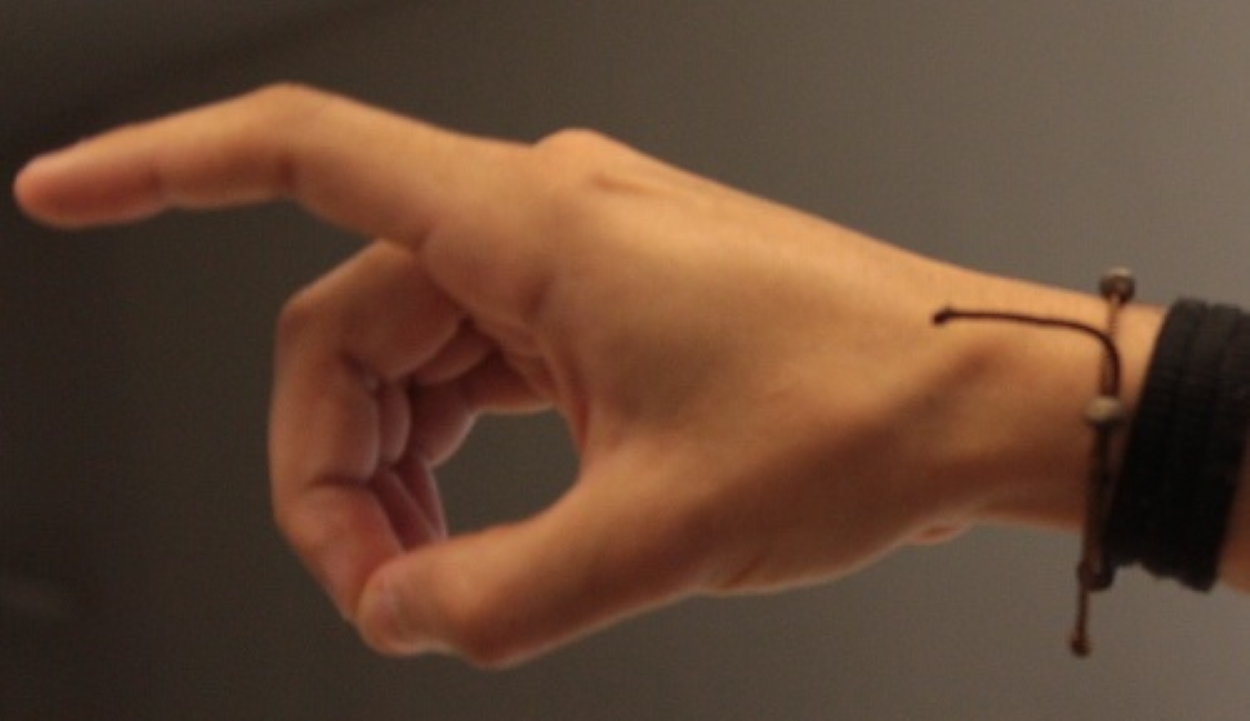
\includegraphics[width=\linewidth]{images/2-recunoasterea-asl/p_dialect2.png}
    \caption{}
    \label{fig:img2}
  \end{subfigure}
  \caption[Dialecte pentru litera P]{\textbf{Dialecte pentru litera P}. \textit{Ambele imagini ilustrează aceeași literă, P, și exemplifică două dialecte diferite, provenind din surse distincte.}}
  \label{fig:p_2_dialecte}
\end{figure}
Literele J și Z au fost eliminate deoarece presupun mișcarea mâinii, iar aplicația noastră analizează un singur cadru independent.


Câte un exemplu sugestiv pentru fiecare literă din setul de date final poate fi analizat în Figura~\ref{fig:ex_per_litera}.
\captionsetup[subfigure]{labelformat=empty}

\begin{figure}[H]

  \centering

  \begin{subfigure}{0.1\textwidth}
    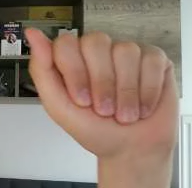
\includegraphics[width=2cm, height=2cm, keepaspectratio=false]{images/7-anexe/a_ex10.png}
    \caption{A}
  \end{subfigure}\hspace{1cm}
  \begin{subfigure}{0.1\textwidth}
    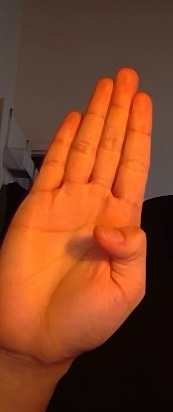
\includegraphics[width=2cm, height=2cm, keepaspectratio=false]{images/7-anexe/b_ex1.jpg}
    \caption{B}
  \end{subfigure}\hspace{1cm}
  \begin{subfigure}{0.1\textwidth}
    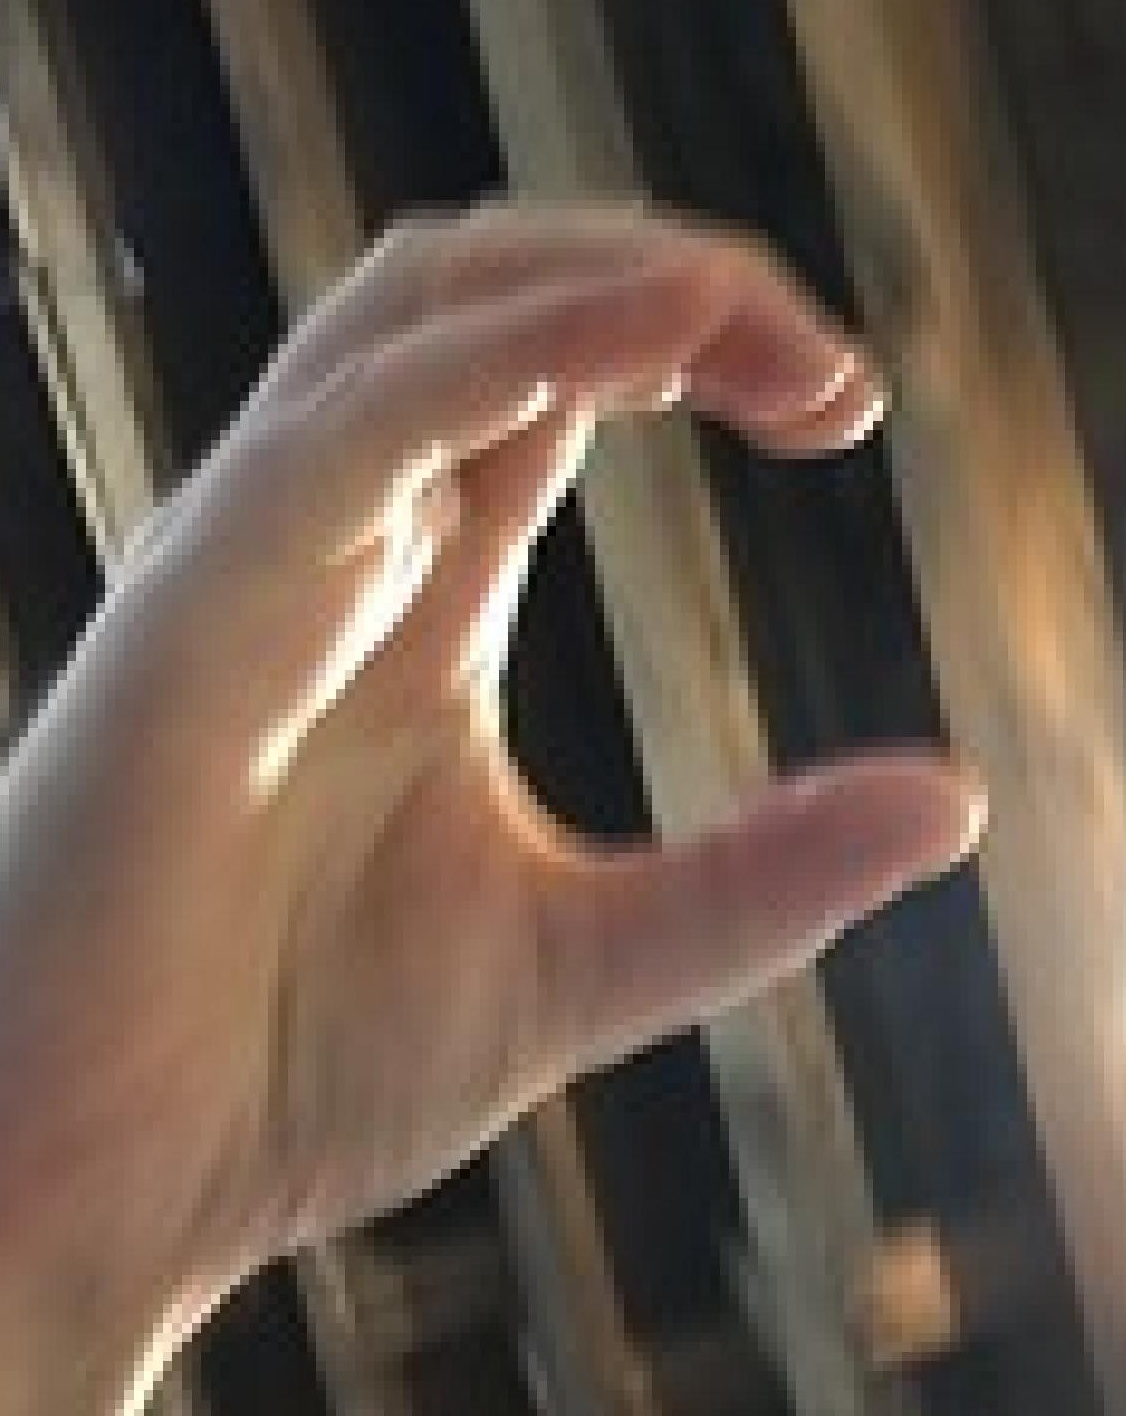
\includegraphics[width=2cm, height=2cm, keepaspectratio=false]{images/7-anexe/c_ex1.jpg}
    \caption{C}
  \end{subfigure}\hspace{1cm}

  

  \begin{subfigure}{0.1\textwidth}
    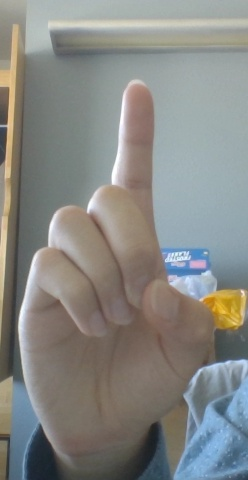
\includegraphics[width=2cm, height=2cm, keepaspectratio=false]{images/7-anexe/d_ex1.jpg}
    \caption{D}
  \end{subfigure}\hspace{1cm}
  \begin{subfigure}{0.1\textwidth}
    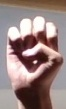
\includegraphics[width=2cm, height=2cm, keepaspectratio=false]{images/7-anexe/e_ex1.jpg}
    \caption{E}
  \end{subfigure}\hspace{1cm}
  \begin{subfigure}{0.1\textwidth}
    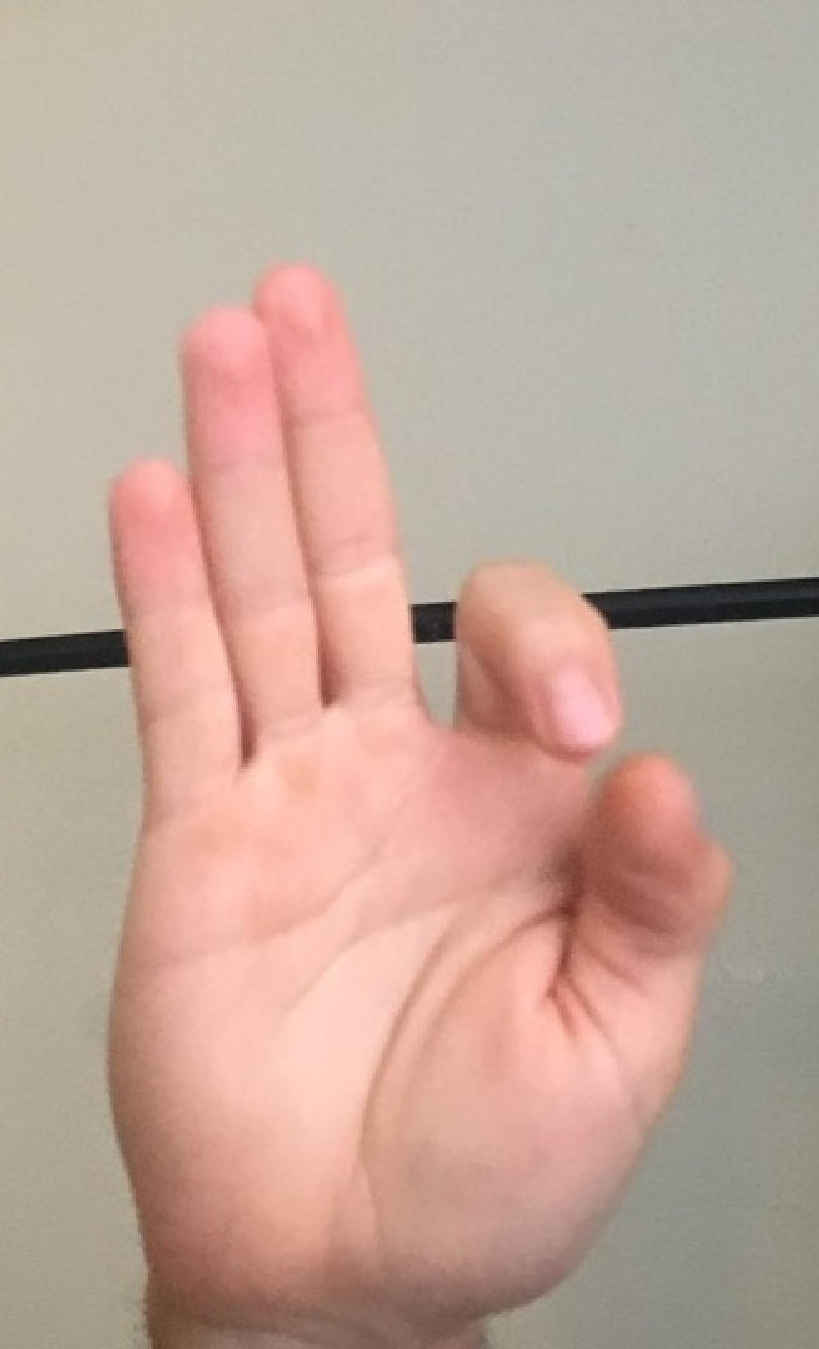
\includegraphics[width=2cm, height=2cm, keepaspectratio=false]{images/7-anexe/f_ex1.jpg}
    \caption{F}
  \end{subfigure}\hspace{1cm}

  

  \begin{subfigure}{0.1\textwidth}
    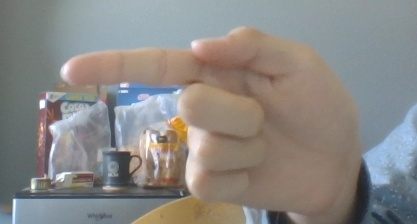
\includegraphics[width=2cm, height=2cm, keepaspectratio=false]{images/7-anexe/g_ex1.jpg}
    \caption{G}
  \end{subfigure}\hspace{1cm}
  \begin{subfigure}{0.1\textwidth}
    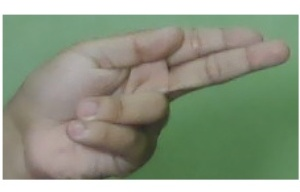
\includegraphics[width=2cm, height=2cm, keepaspectratio=false]{images/7-anexe/h_ex1.jpg}
    \caption{H}
  \end{subfigure}\hspace{1cm}
  \begin{subfigure}{0.1\textwidth}
    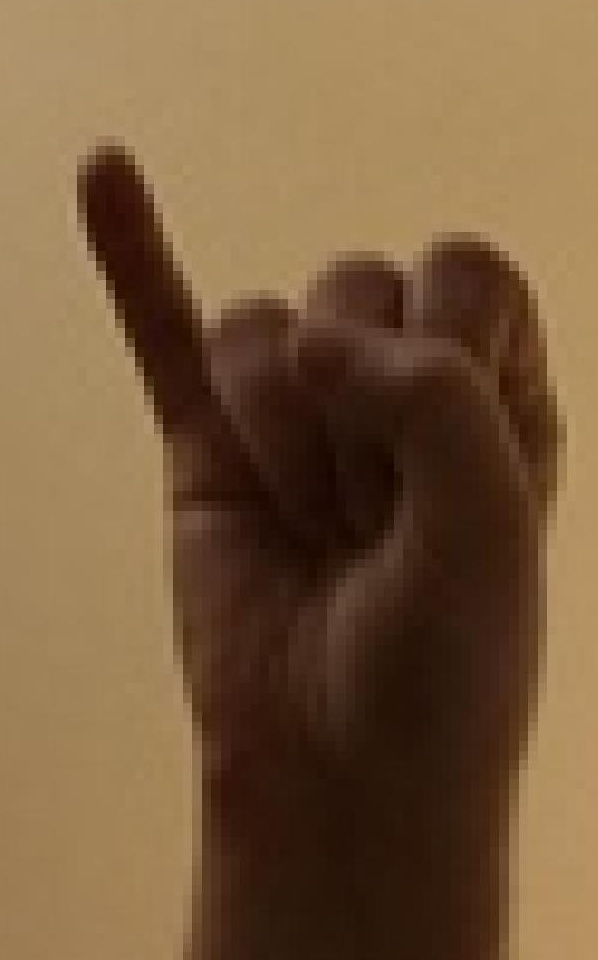
\includegraphics[width=2cm, height=2cm, keepaspectratio=false]{images/7-anexe/i_ex1.jpg}
    \caption{I}
  \end{subfigure}\hspace{1cm}
    
    \begin{subfigure}{0.1\textwidth}
    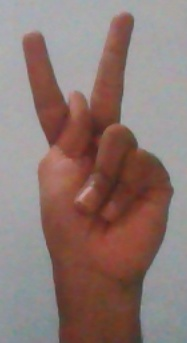
\includegraphics[width=2cm, height=2cm, keepaspectratio=false]{images/7-anexe/k_ex1.jpg}
    \caption{K}
  \end{subfigure}\hspace{1cm}
  \begin{subfigure}{0.1\textwidth}
    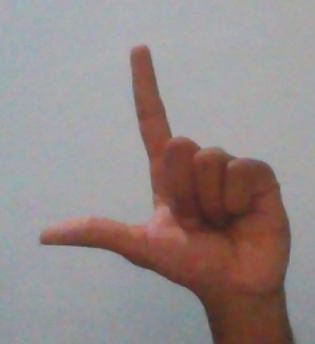
\includegraphics[width=2cm, height=2cm, keepaspectratio=false]{images/7-anexe/l_ex1.jpg}
    \caption{L}
  \end{subfigure}\hspace{1cm}
  \begin{subfigure}{0.1\textwidth}
    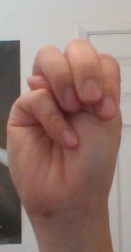
\includegraphics[width=2cm, height=2cm, keepaspectratio=false]{images/7-anexe/m_ex1.jpg}
    \caption{M}
  \end{subfigure}\hspace{1cm}

  

  \begin{subfigure}{0.1\textwidth}
    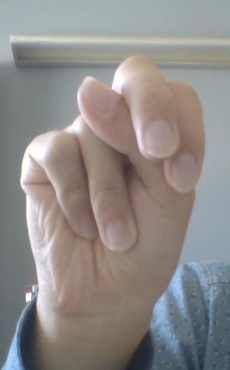
\includegraphics[width=2cm, height=2cm, keepaspectratio=false]{images/7-anexe/n_ex1.jpg}
    \caption{N}
  \end{subfigure}\hspace{1cm}
  \begin{subfigure}{0.1\textwidth}
    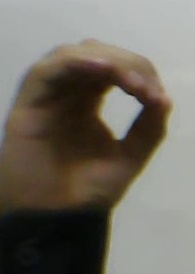
\includegraphics[width=2cm, height=2cm, keepaspectratio=false]{images/7-anexe/o_ex1.jpg}
    \caption{O}
  \end{subfigure}\hspace{1cm}
  \begin{subfigure}{0.1\textwidth}
    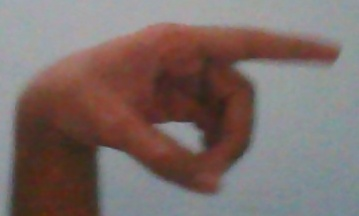
\includegraphics[width=2cm, height=2cm, keepaspectratio=false]{images/7-anexe/p_ex1.jpg}
    \caption{P}
  \end{subfigure}\hspace{1cm}

  

  \begin{subfigure}{0.1\textwidth}
    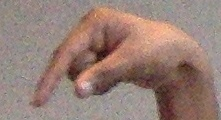
\includegraphics[width=2cm, height=2cm, keepaspectratio=false]{images/7-anexe/q_ex1.jpg}
    \caption{Q}
  \end{subfigure}\hspace{1cm}
  \begin{subfigure}{0.1\textwidth}
    
\includegraphics[width=2cm, height=2cm, keepaspectratio=false]{images/7-anexe/r_ex1.jpg}
    \caption{R}
  \end{subfigure}\hspace{1cm}
  \begin{subfigure}{0.1\textwidth}
    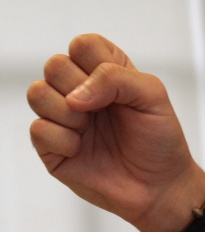
\includegraphics[width=2cm, height=2cm, keepaspectratio=false]{images/7-anexe/s_ex1.JPG}
    \caption{S}
  \end{subfigure}\hspace{1cm}

    \begin{subfigure}{0.1\textwidth}
    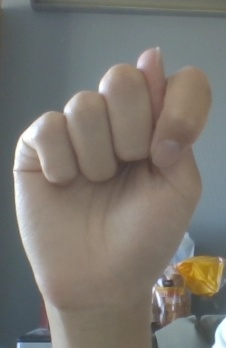
\includegraphics[width=2cm, height=2cm, keepaspectratio=false]{images/7-anexe/t_ex1.jpg}
    \caption{T}
  \end{subfigure}\hspace{1cm}
  \begin{subfigure}{0.1\textwidth}
    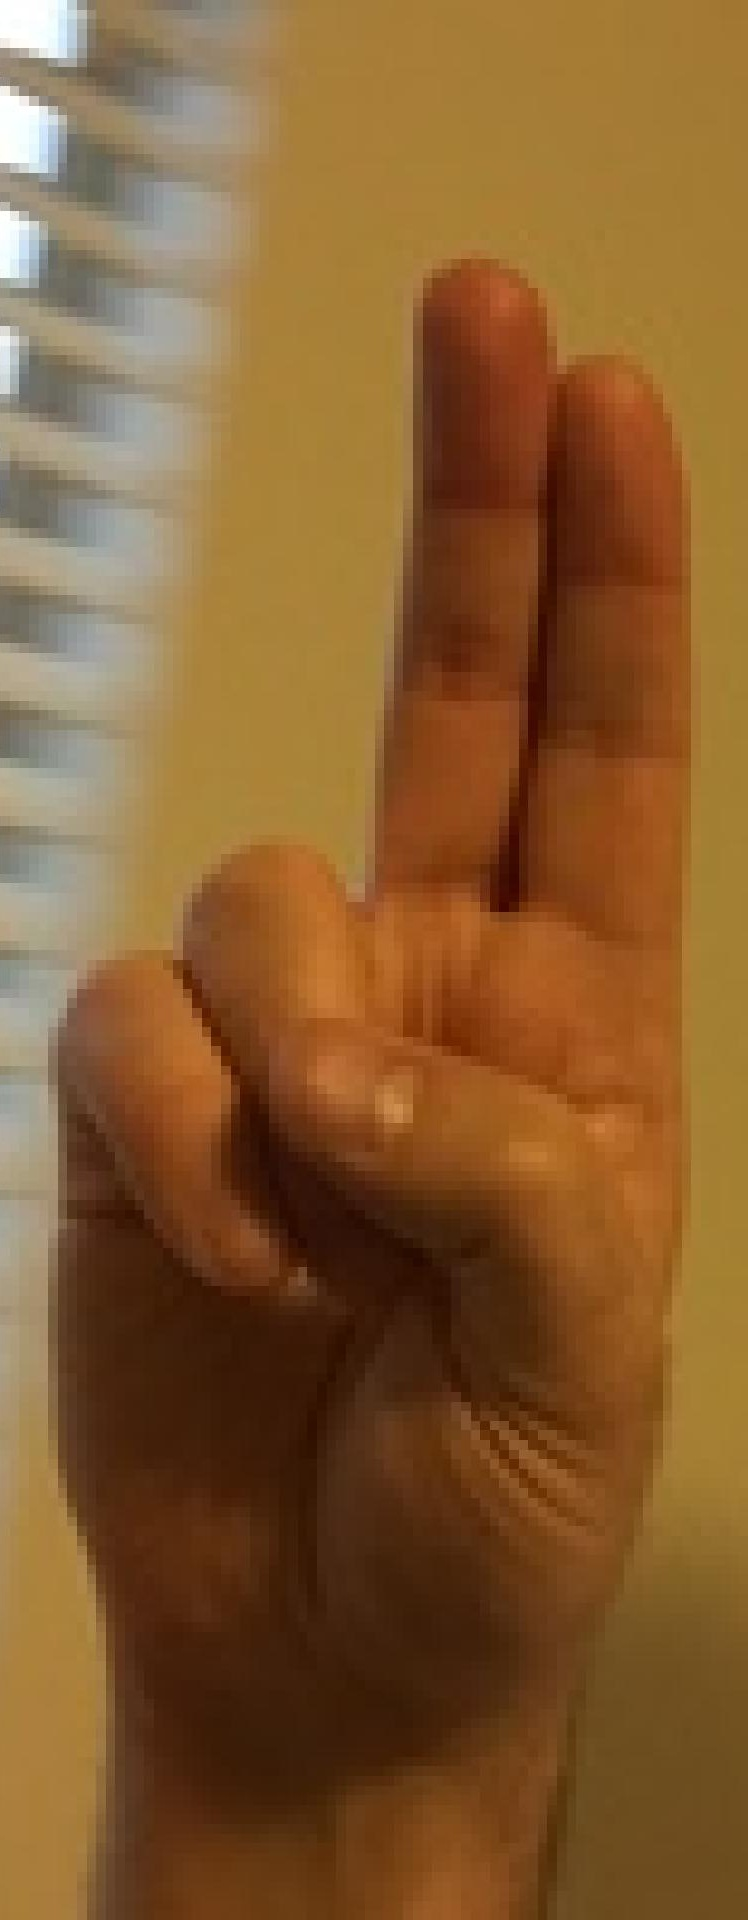
\includegraphics[width=2cm, height=2cm, keepaspectratio=false]{images/7-anexe/u_ex1.jpg}
    \caption{U}
  \end{subfigure}\hspace{1cm}
  \begin{subfigure}{0.1\textwidth}
    
\includegraphics[width=2cm, height=2cm, keepaspectratio=false]{images/7-anexe/v_ex1.jpg}
    \caption{V}
  \end{subfigure}\hspace{1cm}

  

  \begin{subfigure}{0.1\textwidth}
    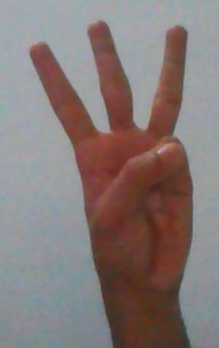
\includegraphics[width=2cm, height=2cm, keepaspectratio=false]{images/7-anexe/w_ex1.jpg}
    \caption{W}
  \end{subfigure}\hspace{1cm}
  \begin{subfigure}{0.1\textwidth}
    
\includegraphics[width=2cm, height=2cm, keepaspectratio=false]{images/7-anexe/x_ex1.png}
    \caption{X}
  \end{subfigure}\hspace{1cm}
  \begin{subfigure}{0.1\textwidth}
    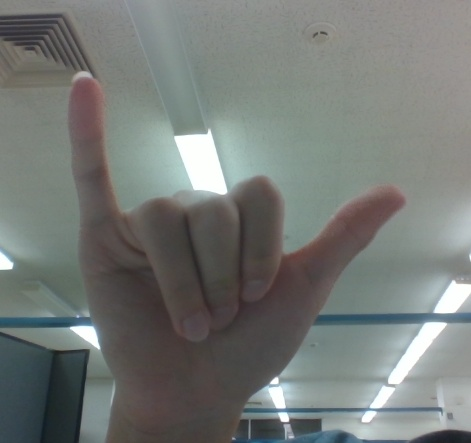
\includegraphics[width=2cm, height=2cm, keepaspectratio=false]{images/7-anexe/y_ex1.jpg}
    \caption{Y}
  \end{subfigure}\hspace{1cm}
  \caption[Literele din setul de date.]{\textbf{Literele din setul de date.} \textit{Ilustrăm câte un exemplu ales aleator, pentru fiecare clasă. Litera situată sub fiecare imagine reprezintă clasa corespunzătoare.}}
  \label{fig:ex_per_litera}
\end{figure}
\captionsetup[subfigure]{labelformat=parens, labelsep=space}

Lucrarea de față este structurată în trei capitole principale, după cum urmează:
\begin{enumerate}
    \item \textbf{Recunoașterea alfabetului ASL} - în acest capitol explicăm procesul care a stat la baza creării setului de date, preprocesarea imaginilor, arhitectura modelului și procesul de antrenare al acestuia. În final, oferim o evaluare experimentală în care analizăm arhitecturile și strategiile nereușite care au contribuit la construirea arhitecturii finale.
    \item \textbf{Aplicația mobilă și infrastructura aplicației} - în acest capitol prezentăm ecranele principale ale aplicației Android, continuând cu o analiză a logicii aplicației și a capacității serverului.
    \item \textbf{Direcții viitoare și concluzii} - în acest ultim capitol recapitulăm procesul științific, analizăm limitările și lipsurile aplicației, posibile soluții privind limitele menționate și oferim direcții viitoare de dezvoltare.
\end{enumerate}
\chapter{Recunoașterea alfabetului ASL}
\label{cap:cap2}

\section{Construirea setului de date}

\textbf{Extragerea cadrelor din videoclipuri}. În cazul seturilor de date formate din clipuri video, a fost utilizat un script \textbf{Python} \cite{python312}, care extrage și salvează cadrele citite cu ajutorul bibliotecii \textbf{OpenCV} \cite{opencv_library}, utilă în procesarea și analiza imaginilor.

\textbf{Extragerea palmei din imagini}. Pentru a extrage mâna, a fost utilizat algoritmul \textbf{MediaPipe Hands}, dezvoltat de \textbf{Google} \cite{zhang2020mediapipehandsondevicerealtime} pentru detecția palmei într-o imagine. Acest pas a fost necesar pentru a elimina zgomotul creat de fundal sau de fețele oamenilor și pentru a aduce palma în prim plan. Transformarea unei imagini în urma aplicării algoritmului poate fi observată în Figura~\ref{fig:before_after_mediapipe}.

În cazul cadrelor extrase din videoclipuri și al palmelor extrase din imagini, imaginile invalide (neclaritate, poziție greșită a mâinii, mână incorectă etc.) au fost eliminate manual.

\begin{figure}[H]
  \centering
  \begin{subfigure}{0.3\textwidth}
  \centering
    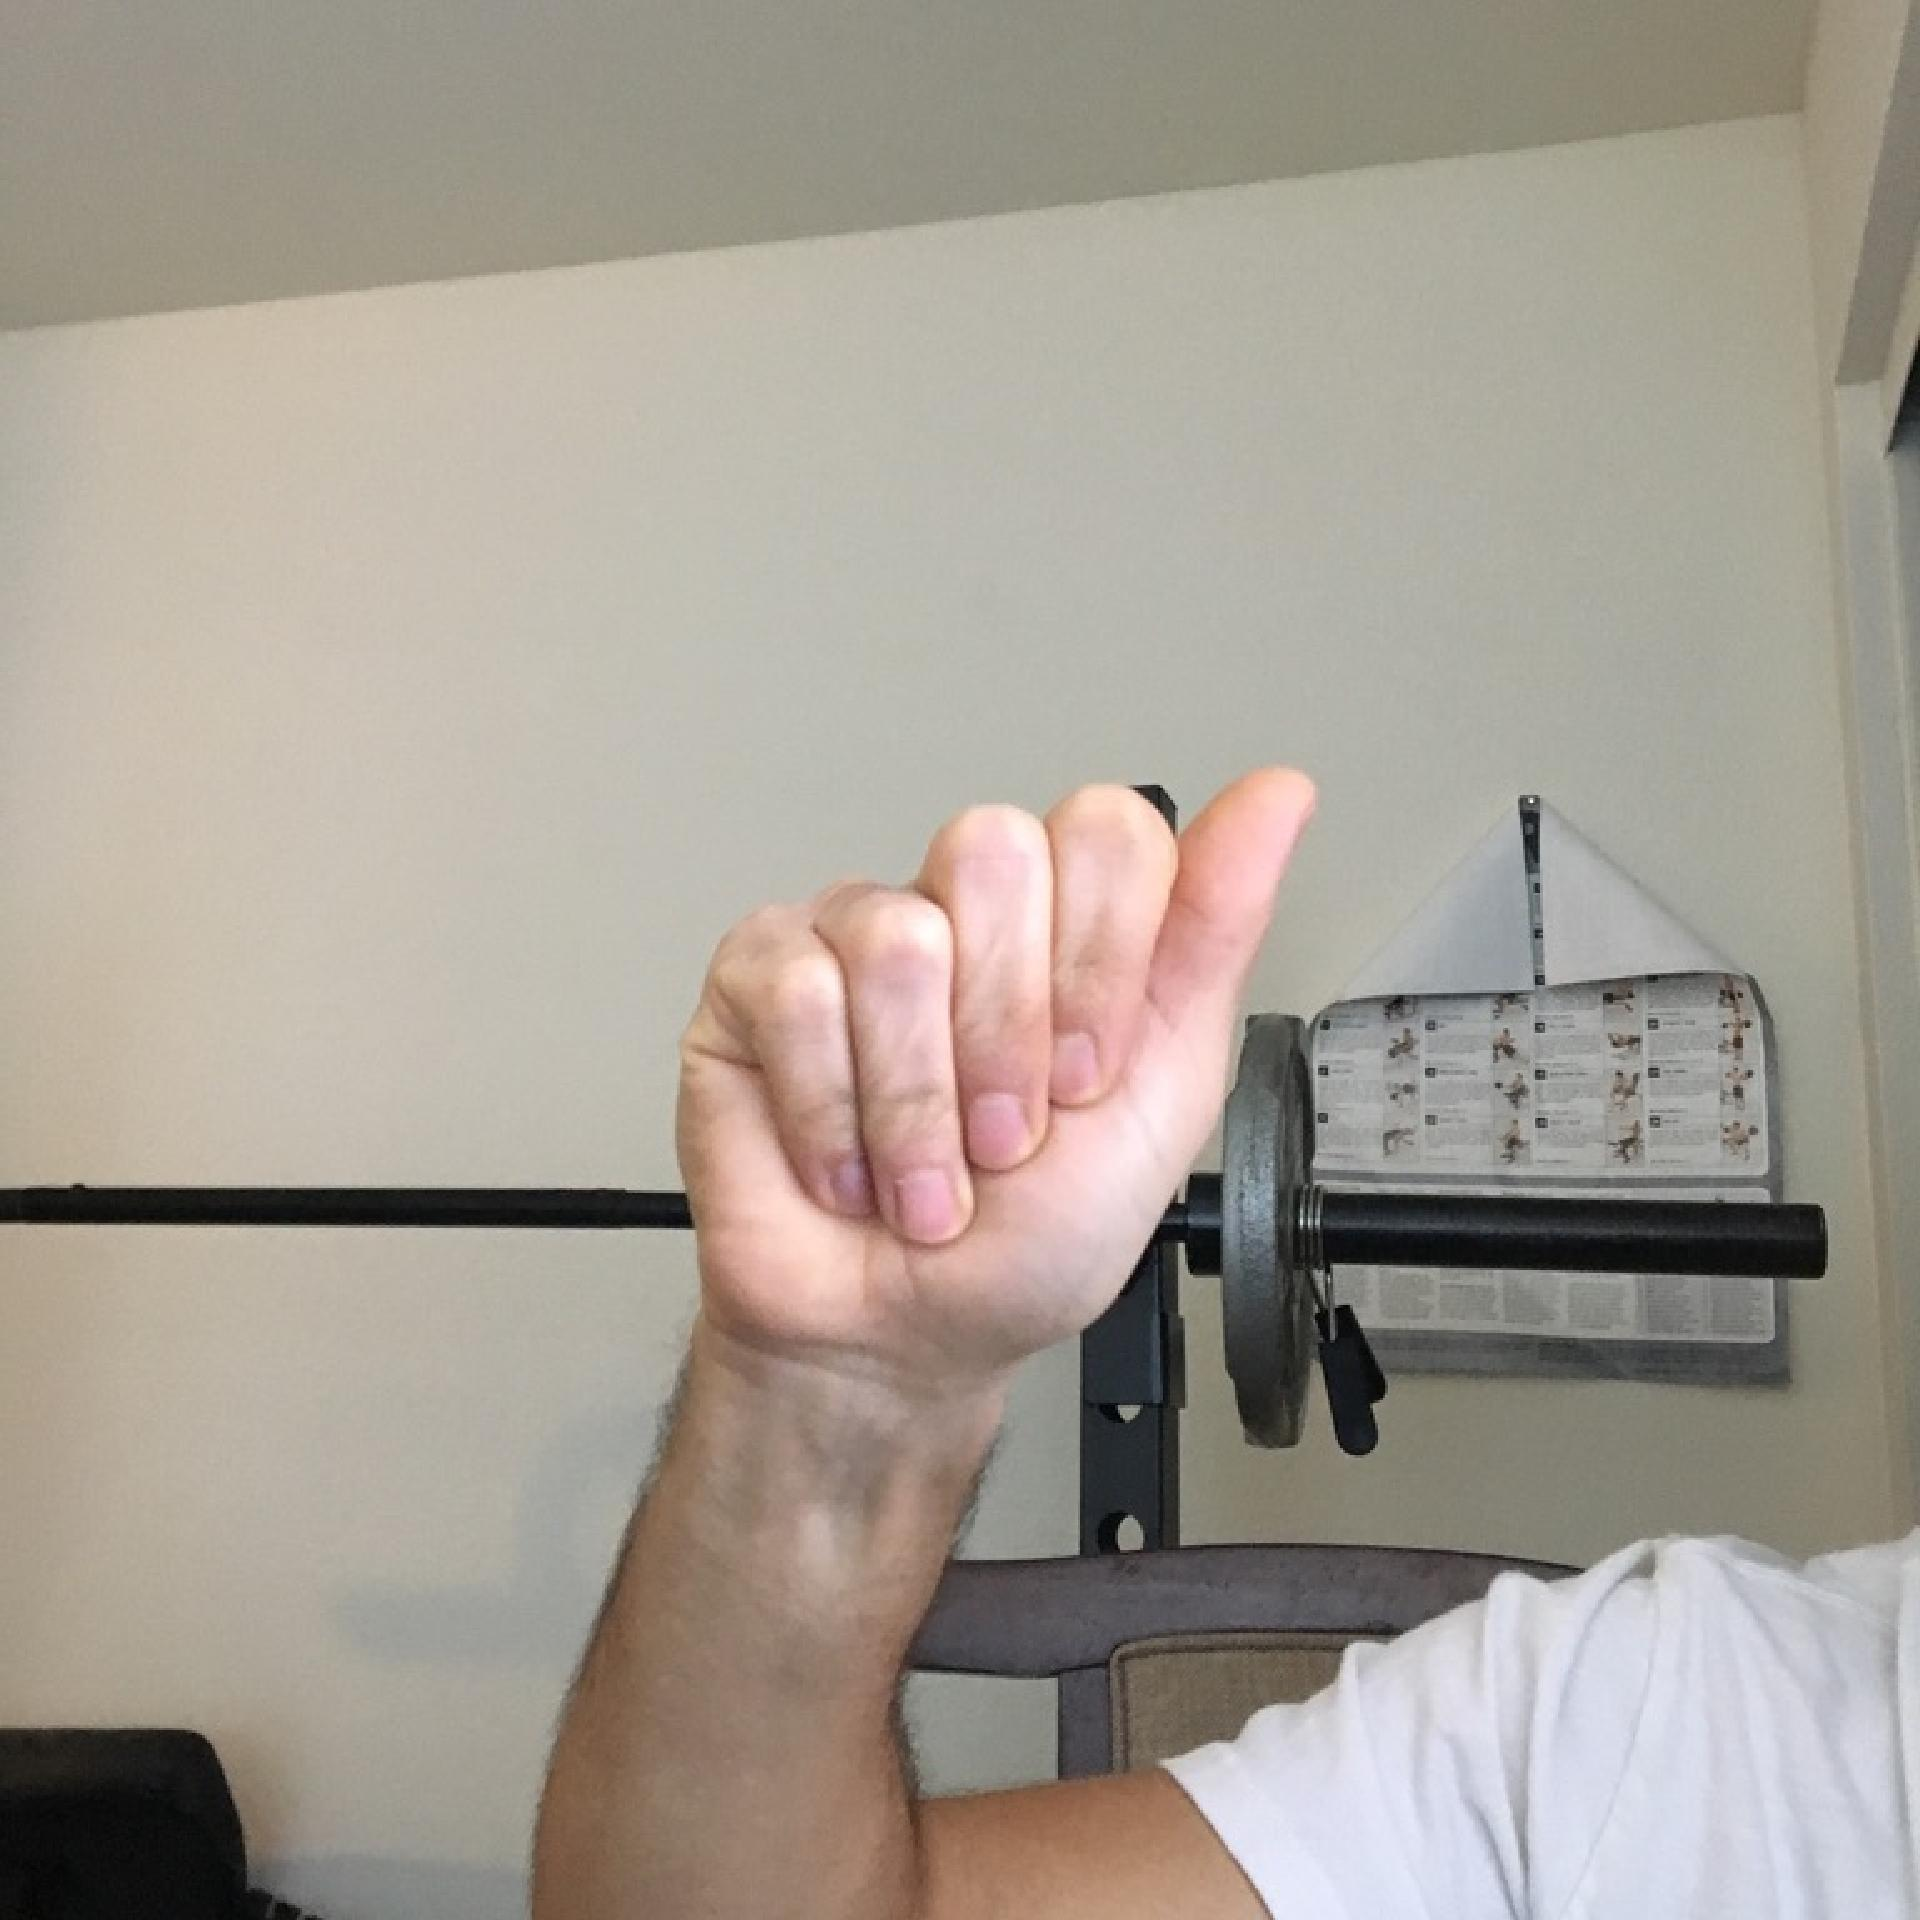
\includegraphics[width=4cm,height=4cm,keepaspectratio]
{images/2-recunoasterea-asl/exemple_litera_a/a_before_mediapipe.jpg}
    \caption{}
  \end{subfigure}
  \hspace{0.1\textwidth}
  \begin{subfigure}{0.3\textwidth}
    \centering
    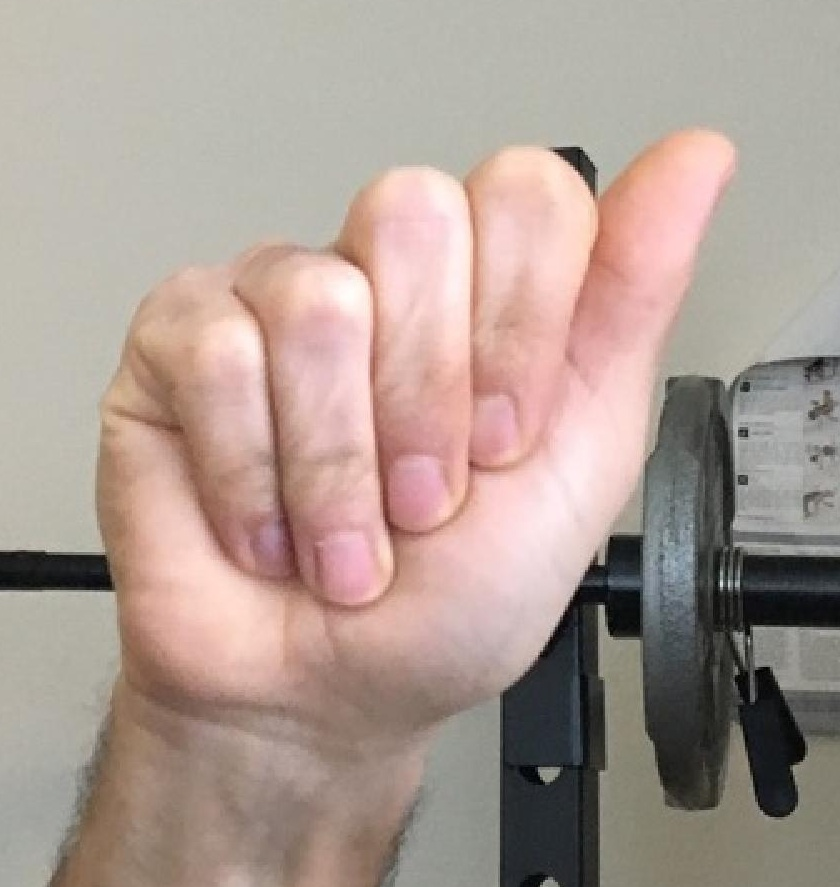
\includegraphics[width=4cm,height=4cm,keepaspectratio]
{images/2-recunoasterea-asl/exemple_litera_a/a_after_mediapipe.jpg}
    \caption{}
  \end{subfigure}
  \caption[Aplicarea MediaPipe Hands]{\textbf{Aplicarea MediaPipe Hands}. \textit{(a) prezintă imaginea originală care servește drept intrare pentru MediaPipe Hands; (b) este imaginea utilizată în antrenare, în urma extragerii acesteia. Se poate observa cum palma devine obiectul principal al imaginii.}}
  \label{fig:before_after_mediapipe}
\end{figure}

\textbf{Împărțirea setului de date}.
Pentru a ne asigura că acuratețea obținută pe seturile de validare și testare reflectă performanța în lumea reală, imaginile sunt împărțite manual, în funcție de sursa lor, astfel încât în seturile de validare și testare să nu existe imagini cu mâini sau fundaluri aflate în setul de de antrenare. În final, avem un total de 36.871 de imagini, împărțite după cum urmează: pentru setul de antrenare sunt alocate 30.450 de imagini, reprezentând 82,58\% din total, pentru setul de validare 3.211 de imagini, reprezentând 8,7\% din total, iar pentru setul de testare 3.210 de imagini, reprezentând 8,7\% din total.

\textbf{Distribuția claselor}. În cazul setului de antrenare, literele subreprezentate sunt M, N și P. Cauza acestei subreprezentări este dificultatea pe care am întâlnit-o în colectarea unui număr suficient de exemple pentru un singur dialect. Cu toate acestea, un număr de aproximativ 1.000 de exemple pentru o clasă este considerat a fi suficient pentru ca modelul să poată învăța trăsăturile importante.

În cazul seturilor de validare și testare, distribuția este aproximativ egală, deoarece clasele nu au necesitat un număr ridicat de exemple, spre deosebire de cele care formează setul de antrenare. Distribuția exactă a seturilor poate fi observată în Figura~\ref{fig:class_distrib}.

\begin{figure}[H]
  \centering
  \begin{subfigure}{0.49\textwidth}
    \centering
    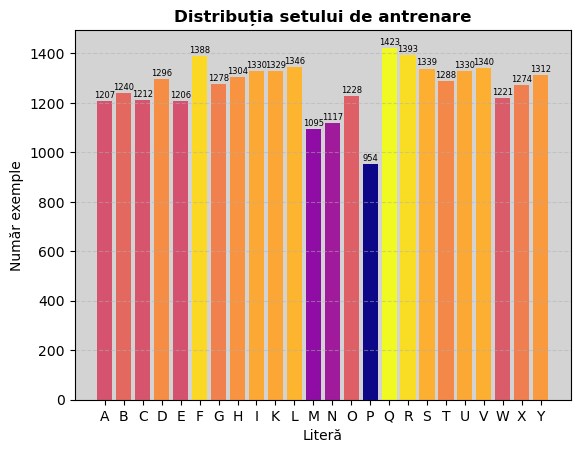
\includegraphics[width=\linewidth]{images/2-recunoasterea-asl/train_classes_distrib.png}
    \caption{}
  \end{subfigure}
  \begin{subfigure}{0.49\textwidth}
    \centering
    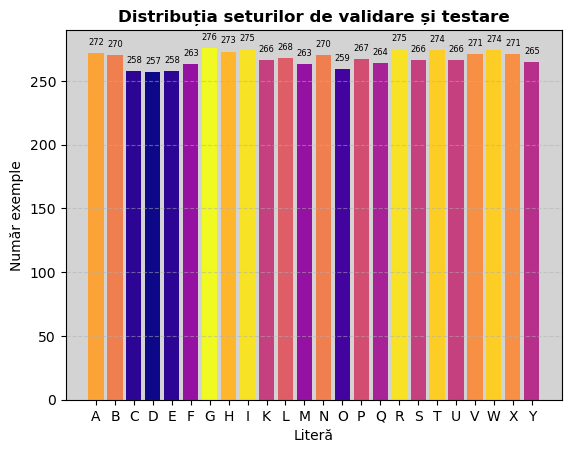
\includegraphics[width=\linewidth]{images/2-recunoasterea-asl/test_val_classes_distrib.png}
    \caption{}
  \end{subfigure}
  \caption[Distribuția claselor]{\textbf{Distribuția claselor}. \textit{(a) ilustrează distribuția setului de antrenare; (b) ilustrează distribuția setului care este împărțit aleator ($seed = 42$), în două seturi: validare și testare.}}
  \label{fig:class_distrib}
\end{figure}

\section{Preprocesarea imaginilor}

\textbf{Preprocesarea setului de antrenare}. Cu scopul de a avea exemple cât mai variate, în special pentru a combate probleme ca \textit{overfitting}-ul, am decis să utilizăm o tehnică numită augmentarea datelor. Efectele clasice (intra-imagine), care acționează independent asupra unei singure imagini, precum răsturnarea, rotirea, aplicarea de estompare sau zgomot, modificarea culorilor sau ștergerea unei porțiuni dintr-o imagine, pot îmbunătăți capacitatea de generalizare a unui model deep, cum ar fi un CNN \cite{data_augment1, data_augment2}. Pe lângă efectele intra-imagine, există și efecte care amestecă două imagini, efecte inter-imagine, cum ar fi \textit{CutMix} \cite{cutmix} și \textit{MixUp} \cite{mixup}.

Pentru efectele clasice, augmentările au fost realizate utilizând biblioteca \textbf{Albumentations} \cite{albumentations}. Augmentările aplicate sunt: răsturnare orizontală cu probabilitatea aplicării de 50\%, rotire între $-15^\circ$ și $15^\circ$ cu o probabilitate de 40\%, estompare cu filtru de dimensiune 3x3 și probabilitate de 30\%, zgomot Gaussian cu abatere standard între 0.05 și 0.07 și o probabilitate de 30\% și trepidație de culoare sau \textit{color jitter} (schimbarea luminozității, contrastului, saturației și nuanței), cu o probabilitate de 40\%. Toate imaginile sunt redimensionate la $224 \times 224$, normalizate folosind media per canal RGB $[0.5797, 0.5104, 0.4846]$ și abatere standard $[0.1804, 0.1845, 0.1883]$, reprezentând media și abaterea standard a setului de antrenare, și în final, transformate în tensori. 

După cum se observă în Figura~\ref{fig:exemplu_efecte_clasice}, efectele aplicate pot ajuta modelul să „înțeleagă” că factori precum culoarea pielii sau poziția exactă a mâinii nu sunt importanți, și mai mult de atât, să se descurce în condiții de luminozitate scăzută și cu imagini de calitate redusă.
 
\begin{figure}[H]
  \centering
 \begin{subfigure}{0.18\textwidth}
      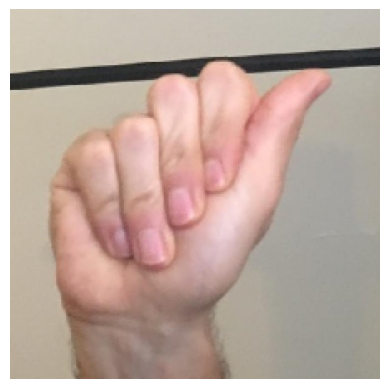
\includegraphics[width=\linewidth]{images/2-recunoasterea-asl/imagine_a_originala.png}
      \caption{}
    \end{subfigure}
    \begin{subfigure}{0.18\textwidth}
      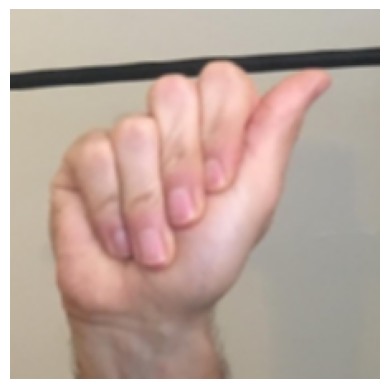
\includegraphics[width=\linewidth]{images/2-recunoasterea-asl/imagine_a_blur.png}
      \caption{}
    \end{subfigure}
    \hspace{0.005\textwidth}
    \begin{subfigure}{0.18\textwidth}
      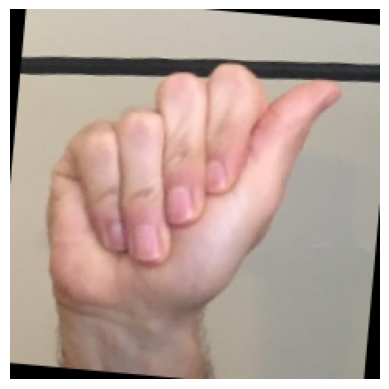
\includegraphics[width=\linewidth]{images/2-recunoasterea-asl/imagine_a_rotate.png}
      \caption{}
    \end{subfigure}
    \hspace{0.005\textwidth}
    \begin{subfigure}{0.18\textwidth}
      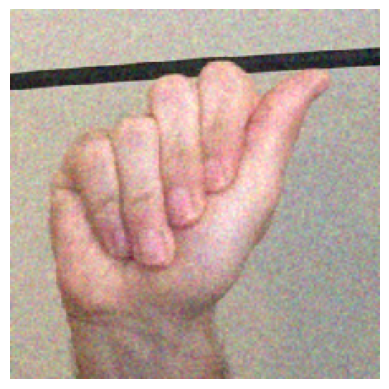
\includegraphics[width=\linewidth]{images/2-recunoasterea-asl/imagine_a_gauss_noise.png}
      \caption{}
    \end{subfigure}
    \hspace{0.005\textwidth}
    \begin{subfigure}{0.18\textwidth}
      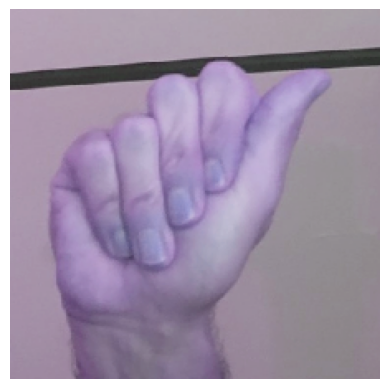
\includegraphics[width=\linewidth]{images/2-recunoasterea-asl/imagine_a_color_jitter.png}
      \caption{}
    \end{subfigure}

  \caption[Efecte intra-imagine]{\textbf{Efecte intra-imagine}. \textit{Ilustrăm efectele aplicate asupra imaginilor, pentru augmentarea setului de antrenare. (a) exemplifică imaginea originală, (b) exemplifică efectul de estompare, (c) exemplifică rotirea, (d) exemplifică zgomotul adăugat, iar (e) exemplifică efectul de color jitter.}}
  \label{fig:exemplu_efecte_clasice}
\end{figure}

În cazul efectelor inter-imagine CutMix și MixUp am utilizat biblioteca \textbf{torchvision} \cite{torchvision2016}. La fiecare încărcare a unui \textit{batch} de date din setul de antrenare, cu ajutorul unui obiect de tip \textit{DataLoader} din biblioteca \textbf{PyTorch} \cite{pytorch}, alegem aleatoriu dintre CutMix sau MixUp, cu o probabilitate de aplicare de 50\%. 

CutMix este definit ca:
\begin{equation}
    \begin{aligned}
        \tilde{x} &= M \odot x_B + (1 - M) \odot x_A \\
        \tilde{y} &= \lambda y_A + (1 - \lambda) y_B
    \end{aligned}
    \label{eq:cutmix}
\end{equation}
unde $\tilde{x}$ este imaginea rezultată, $x_B$ și $x_A$ sunt imaginile sursă care vor fi combinate, iar $M$ este masca binară care va fi înmulțită element cu element ($\odot$) cu imaginile sursă. $\tilde{y}$ este eticheta \textit{soft}, iar $\lambda$ reprezintă ponderea fiecărei imagini în imaginea finală.

MixUp este definit ca:
\begin{equation}
    \begin{aligned}
        \tilde{x} &= \lambda x_A + (1 - \lambda) x_B \\
        \tilde{y} &= \lambda y_A + (1 - \lambda) y_B
    \end{aligned}
    \label{eq:cutmix}
\end{equation}
unde $\tilde{x}$ este imaginea rezultată, $x_A$ și $x_B$ sunt imaginile sursă care vor fi combinate, iar $\lambda$ este un coeficient ales aleator, care controlează proporția fiecărei imagini. $\tilde{y}$ este la fel ca și în cazul ecuației pentru CutMix.

Este important de menționat că, în cazul nostru, păstrăm din tehnica CutMix și MixUp doar combinarea imaginilor, iar eticheta atribuită corespunde clasei dominante din imaginea compusă.

Pentru a vizualiza efectele aplicate asupra a două imagini, vezi Figura~\ref{fig:exemplu_efecte_avansate}.

\begin{figure}[H]
  \centering
    \begin{subfigure}{0.22\textwidth}
      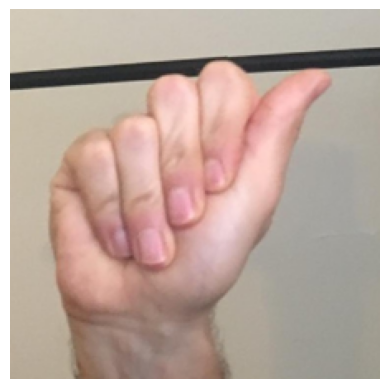
\includegraphics[width=\linewidth]{images/2-recunoasterea-asl/ctmx_mxup_orig_1.png}
      \caption{}
    \end{subfigure}
    \hspace{0.001\textwidth}
    \begin{subfigure}{0.22\textwidth}
      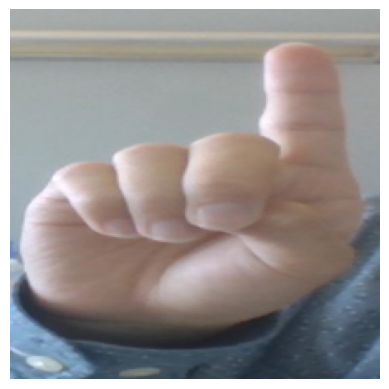
\includegraphics[width=\linewidth]{images/2-recunoasterea-asl/ctmx_mxup_orig_2.png}
      \caption{}
    \end{subfigure}
    \hspace{0.001\textwidth}
    \begin{subfigure}{0.25\textwidth}
      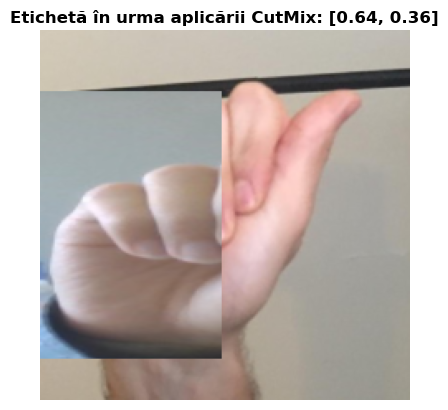
\includegraphics[width=\linewidth]{images/2-recunoasterea-asl/ctmx_img_1.png}
      \caption{}
    \end{subfigure}
    \hspace{0.001\textwidth}
    \begin{subfigure}{0.25\textwidth}
      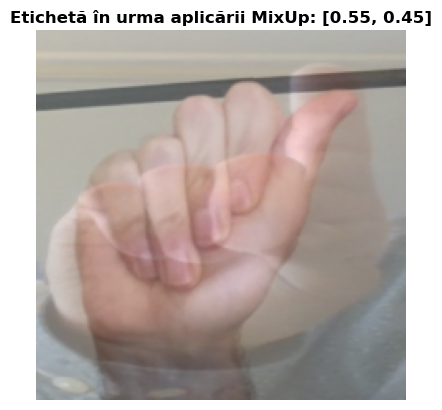
\includegraphics[width=\linewidth]{images/2-recunoasterea-asl/mxup_img_1.png}
      \caption{}
    \end{subfigure}

  \caption[CutMix și MixUp]{\textbf{CutMix și MixUp}. \textit{Ilustrăm efectele CutMix și MixUp. (a) și (b) reprezintă două exemple din două clase distincte; (c) exemplifică efectul CutMix, unde clasa din (a) are o pondere de 0.64, iar (b) are o pondere de 0.36; (d) exemplifică efectul MixUp, unde clasa (a) are o pondere de 0.55, iar clasa (b) are o pondere de 0.45.}}
  \label{fig:exemplu_efecte_avansate}
\end{figure}

\textbf{Preprocesarea seturilor de validare și testare}. În cazul acestor două seturi, imaginea originală este redimensionată 
la $224 \times 224$, normalizată cu media și abaterea standard a setului de antrenare și transformată în tensori.

\section{Arhitectura modelului}

Arhitectura creată pentru acest studiu a fost inspirată din mai multe arhitecturi revoluționare, precum VGG \cite{vggnet} de unde a fost preluată ideea utilizării de bloc (mai multe straturi) convoluțional, urmat de un strat de \textit{max pooling}, tehnică care reduce dimensiunea hărților de activare.

În plus, arhitecura a fost inspirată de ResNet \cite{resnet}, prin inserarea unor straturi convoluționale succesive care păstrează numărul de canale, consolidând și rafinând trăsăturile extrase în ultima extindere. Din aceeași arhitectură, a fost inspirată și inserarea straturilor de \textit{batch normalization} după straturile convoluționale, cu scopul de a accelerara procesul de învățare, permițând utilizarea unei rate de învățare mai mare, și de a oferi o ușoară regularizare prin reducerea variațiilor
mari \cite{batch_norm}. În final, a fost preluată și tehnica de \textit{adaptive average pooling}, prin care este redusă înălțimea și lățimea imaginii la $1\times1$, păstrând adâncimea (numărul canalelor).

Modelul este format din 12 straturi convoluționale, fiecare urmat de câte un strat de batch normalization și activat cu ajutorul funcției de activare ReLU, fiind una dintre cele mai utilizate funcții de activare în cazul modelelor de tip CNN, deoarece oferă acuratețe ridicată în sarcini precum clasificarea imaginilor \cite{relu1, relu2}. În final, este prezent un clasificator format din două straturi complet conectate (dense). Straturile convoluționale sunt împărțite în cinci blocuri care sunt explicate în continuare. Pentru o mai bună înțelegere a arhitecturii și a explicației ce urmează, vezi Figura~\ref{fig:diagrama_vladimirnet}.

\begin{figure}[H]
  \centering
  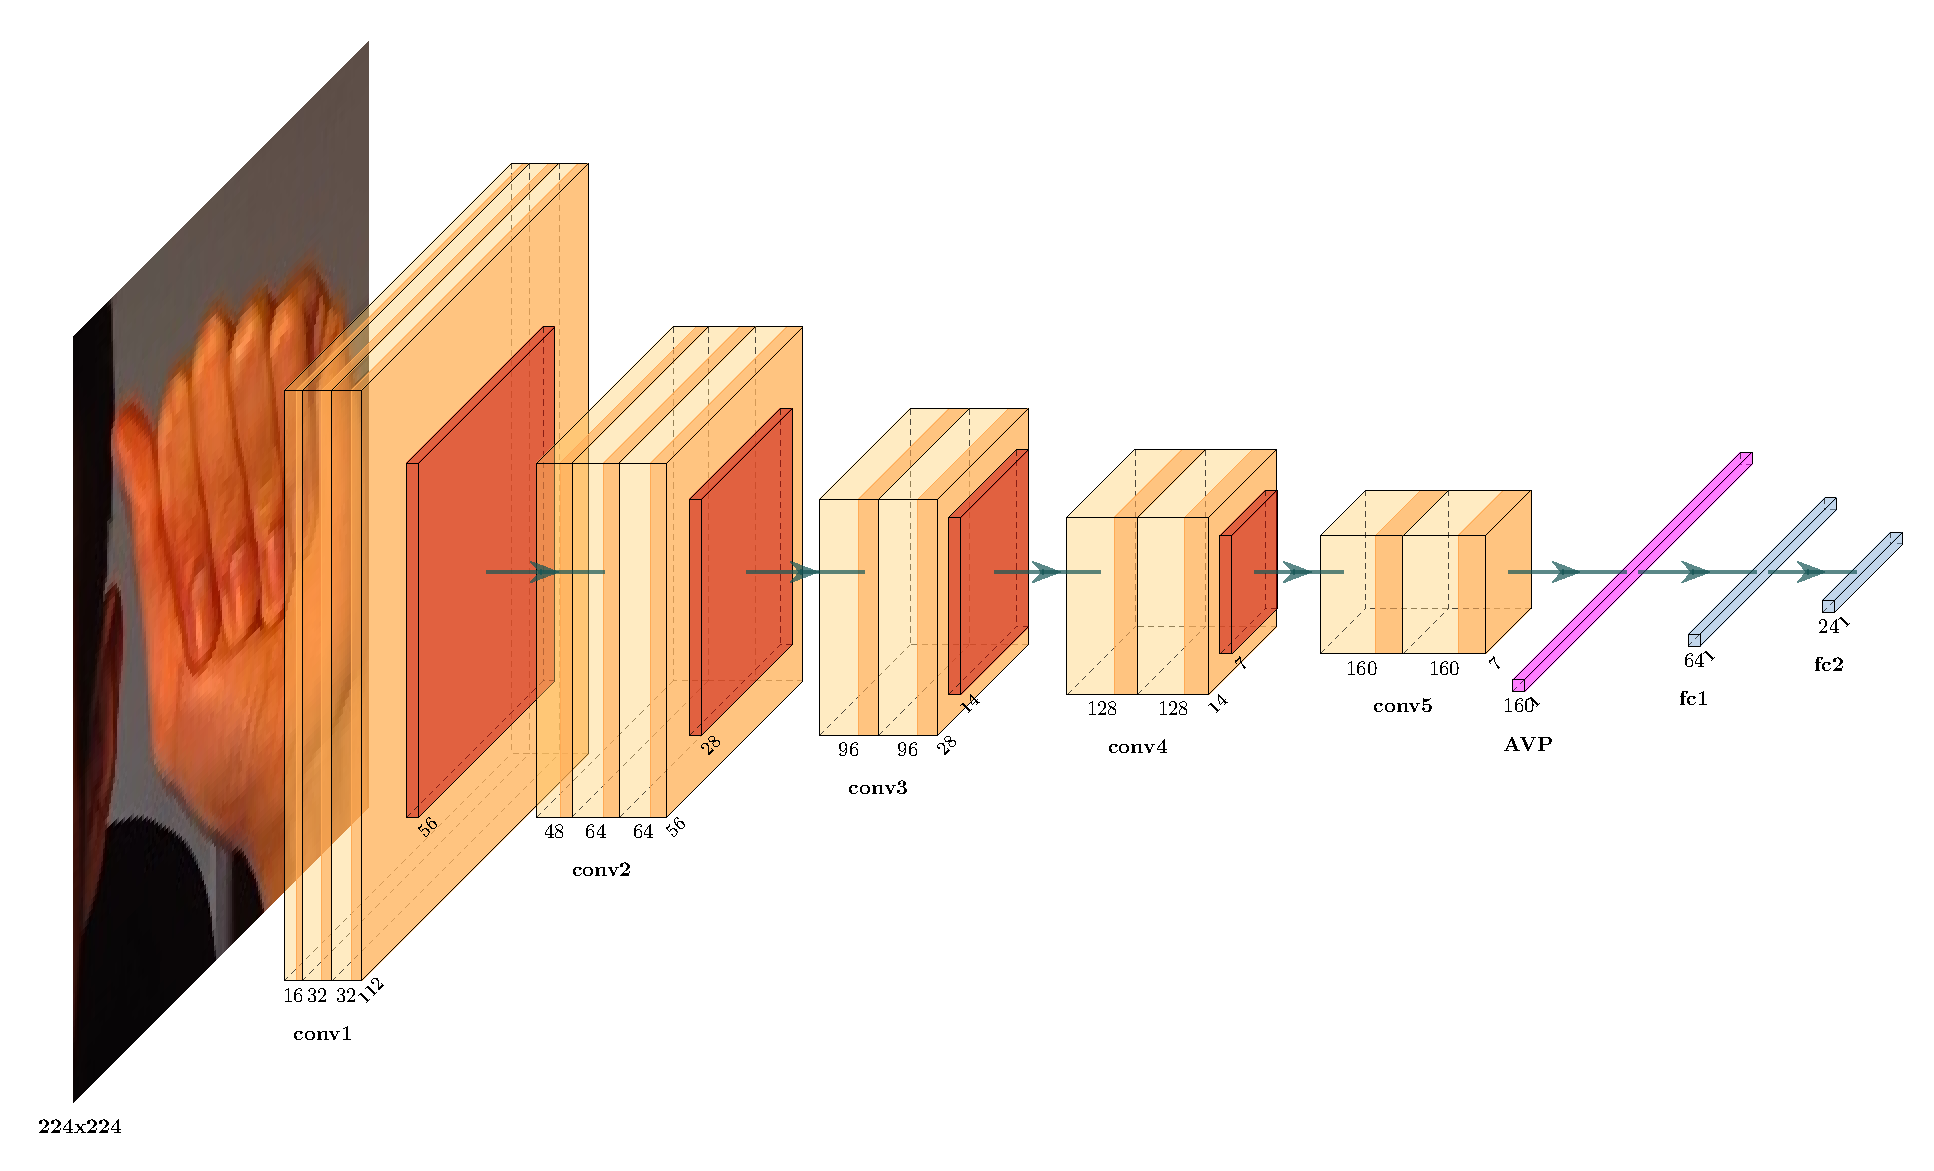
\includegraphics[width=\textwidth]{images/2-recunoasterea-asl/VladimirNetArchitecture.pdf}
  \caption[Arhitectura VladimirNet]{\textbf{Arhitectura VladimirNet}. \textit{Ilustrăm arhitectura modelului utilizat în lucrare, denumită \textbf{VladimirNet}. Conține un număr total de 927.496 de parametri. Prima imagine din stânga reprezintă imaginea care este transmisă modelului, cu dimensiunea inițială de 224 \times 224. Blocurile convoluționale sunt notate cu conv1, conv2, conv3 conv4, conv5. Fiecare strat este evidențiat cu galben transparent și are notat dedesubt numărul de canale în urma aplicării operației de convoluție. Straturile de batch normalization și ReLU sunt ilustrate cu portocaliu, iar culoarea roșie indică operația de max pooling. AVP reprezintă operația de adaptive average pooling. Fc1 și fc2 sunt straturile dense ale clasificatorului. Diagrama a fost construită cu ajutorul bibliotecii \LaTeX, \textbf{PlotNeuralNet}} \cite{haris_iqbal_2018_2526396}.}
  \label{fig:diagrama_vladimirnet}
\end{figure}

\begin{enumerate}
    \item Primul bloc este format din trei straturi convoluționale. Primul strat extinde numărul canalelor de la trei (RGB) la 16, crescând adâncimea și micșorând imaginea la $112 \times 112$, utilizând kernel de $5 \times 5$ și $stride = 2$ cu $padding = 2$. Dimensiunea este redusă la $112 \times 112$ pentru a nu consuma prea multă memorie la început, având în vedere dimensiunea kernel-ului de $5 \times 5$ care poate fi mai costisitor din punct de vedere computațional. Al doilea strat din blocul curent extinde din nou numărul de canale la 32 și utilizează tot un kernel de $5\times 5$, concentrându-se în continuare pe caracteristici generale. Ultimul strat, la fel ca toate straturile din finalul blocurilor convoluționale ale arhitecturii, nu adâncește imaginea, ci păstrează numărul de canale din stratul anterior, însă de data aceasta folosind un kernel de $3 \times 3$. Scopul ultimului strat este rafinarea și consolidarea trăsăturilor învățate pâna atunci, înainte de stratul de max pooling, cu rolul de a reduce dimensiunea spațială la jumătate. Fiecare bloc convoluțional din cele descrise în continuare este urmat de un strat de max pooling, cu excepția ultimului. 
    \item Al doilea bloc funcționează pe același principiu: 3 straturi convoluționale, ultimul păstrând numărul de canale, însă de acum înainte toate straturile utilizează un kernel cu dimensiunea de $3 \times 3$.
    \item Al treilea, al patrulea și al cincilea bloc conțin numai 2 straturi convoluționale, pentru a controla complexitatea modelului, având în vedere că ultimul strat atinge un număr de 160 de canale.
    \item Ultimul bloc convoluțional nu mai este urmat de max pooling, ci de adaptive average pooling, strat care reduce dimensiunea spațială a fiecărei hărți la $1 \times 1$, rezultând un vector cu $160$ de valori.
    \item În final, vectorul rezultat este transmis către clasificatorul format din două straturi complet conectate. Primul strat este urmat de ReLU și un strat de \textit{dropout} cu $p=0.45$, care dezactivează aleatoriu $45\%$ dintre neuroni și conexiunile acestora, metodă necesară pentru a combate overfitting-ul \cite{dropout1, dropout2}. Ultimul strat dens este cel care ne oferă predicția.
\end{enumerate}
 
De asemenea, este important să menționăm că ponderile sunt inițializate prin metoda \textit{Kaiming}, care folosește valori dintr-o distribuție normală. Scopul acestei inițializări este de a evita gradienți care tind spre 0 (\textit{vanishing gradient)} sau care „explodează” (\textit{exploding gradient)} 
\cite{kaiming_w_init}.

\section{Antrenarea modelului}
Antrenarea modelului a fost realizată în platforma \textbf{Google Colab} \cite{colab}, folosind un \textit{GPU} \textbf{NVIDIA L4}.

\textbf{Funcția de pierdere}. Pentru evaluarea predicțiilor oferite de către model, este utilizată entropia încrucișată (în engl. \textit{Cross Entropy}) implementată cu ajutorul clasei \textit{CrossEntropyLoss} din PyTorch, după formula:

\begin{equation}
    L = - \sum_{i=1}^{C}y_i \cdot \log(\hat{y}_i)
\end{equation}
unde $C$ este numărul de clase posibile, $y_i$ reprezintă vectorul \textit{one-hot} a etichetei corecte, iar $\hat{y}_i$ este vectorul rezultat din ultimul strat dens, asupra căruia este aplicată funcția de activare \textit{softmax}.

Ca metodă de regularizare, vom folosi și o tehnică denumită \textit{label smoothing} (netezirea etichetelor) \cite{label_smooth}, astfel încât $y_i$, vectorul one-hot \textit{hard} utilizat de funcția cross entropy, este înlocuit cu unul soft care îndepărtează modelul de predicții excesiv de încrezătoare.


\textbf{Algoritmul de optimizare}. Pentru antrenarea modelului, s-a hotărât utilizarea algoritmului de optimizare \textit{AdamW} \cite{adamw_article}, bazat pe Adam (Adaptive Moment Estimation) \cite{adam_article}. Îmbunătățirea adusă de către AdamW algoritmului de optimizare Adam constă în decuplarea 
penalizării ponderilor mari (în engl. \textit{weight decay}) de calculul gradientului, astfel încât formula pentru actualizarea ponderilor este următoarea: 

\begin{equation}
    \theta_{t+1} = \theta_t - \eta \cdot \left(\frac{\hat{m}_t}{\sqrt{\hat{v}_t} + \epsilon} + \lambda \cdot \theta_t\right)
\end{equation}
unde $\theta_{t}$ sunt ponderile în pasul $t$, $\eta$ este rata de învățare, $\hat{m}_t$ este media exponențială a gradientelor în pasul $t$, $\hat{v}_t$ este  media exponențială a pătratelor gradientelor în pasul $t$, iar $\lambda$ reprezintă factorul de penalizare a greutăților.


\textbf{Hiperparametri}. Pentru optimizator, am ales o rată de învățare $\eta = 1\times 10^{-3}$, aceasta fiind valoarea implicită din clasa \textit{AdamW} a bibliotecii PyTorch. Pe parcursul învățării, $\eta$ este ajustat treptat, la final având o valoare de $1\times10^{-5}$. Ajustarea este facilitată de clasa \textit{CosineAnnealingLR} din PyTorch, care actualizează $\eta$ la finalul fiecărui batch. Scopul acestei ajustări este de a scoate modelul din anumite minime locale nedorite, iar pe parcursul învățarii, actualizările parametrilor să fie din ce în ce mai fine.

După cum am menționat mai devreme, etichetele sunt „netezite” înainte de a fi oferite funcției de pieredere, cu un factor de netezire $\epsilon = 0.15$, penalizând predicțiile excesiv de încrezătoare.

Timpul de antrenament este de 60 de epoci, cu mărimea batch-ului de 64 de exemple.

Pentru weight decay, utilizăm o valoare de $1 \times 10^{-6}$. Valoarea implicită pentru weight decay este de $1\times10^{-2}$, însă o valoare așa ridicată conduce către o învățare mai lentă.

\section{Evaluarea modelului}

În timpul antrenării, la finalul fiecărei epoci, performanța modelului era evaluată pe setul de validare. Modelul a fost salvat în fiecare punct maxim al acurateții obținute pe setul de validare.

Evaluările au fost create și vizualizate cu ajutorul bibliotecilor \textbf{scikit-learn} \cite{scikit-learn}, \textbf{Matplotlib} \cite{matplotlib} și \textbf{seaborn} \cite{seaborn}.

Putem observa în Figura~\ref{fig:train_val_acc}
evoluția modelului pe parcursul celor 60 de epoci. Acuratețea maximă pe setul de antrenare este de $92,45\%$, iar pe setul de validare de $92,27\%$. Datorită augmentărilor puternice și dificultății setului de antrenare, comparativ cu cel de validare, acuratețea setului de validare s-a menținut aproape constant deasupra acurateții setului de antrenare, iar spre final, acuratețea setului de antrenare ajungând să stagneze, cu o ușoară tendință descendentă. 

În Figura~\ref{fig:train_val_loss} putem observa cum funcția de pierdere scade treptat, indicând o învățare continuă.


\begin{figure}[H]
  \centering
  \begin{subfigure}{0.49\textwidth}
    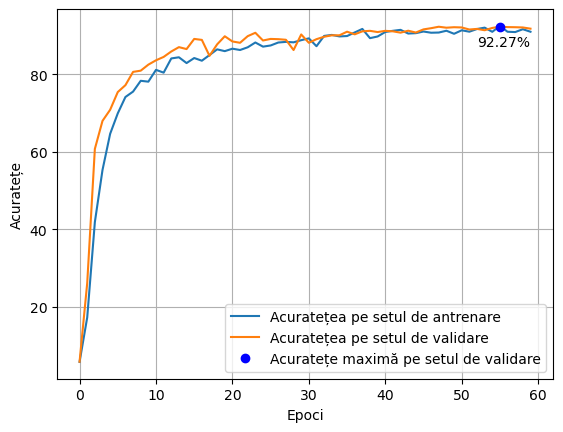
\includegraphics[width=\linewidth]{images/2-recunoasterea-asl/train_val_accs.png}
    \caption{}
    \label{fig:train_val_acc}
  \end{subfigure}
  \begin{subfigure}{0.49\textwidth}
    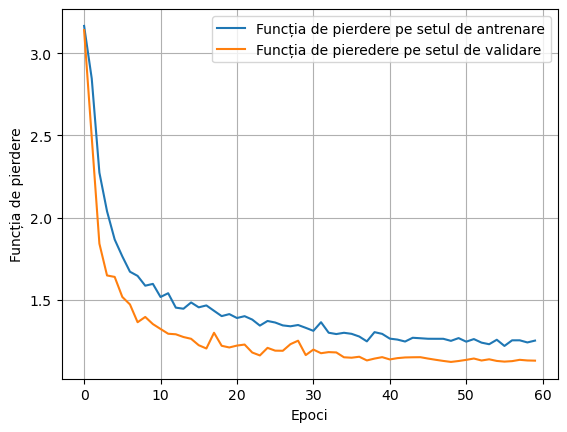
\includegraphics[width=\linewidth]{images/2-recunoasterea-asl/train_val_loss.png}
    \caption{}
    \label{fig:train_val_loss}
  \end{subfigure}
  \caption[Vizualizarea antrenării]{\textbf{Vizualizarea antrenării}. \textit{(a) ilustrează evoluția acurateții pe parcursul celor 60 de epoci de antrenare; (b) ilustrează evoluția funcției de pierdere pe parcursul antrenării.}}
  \label{fig:train_val_acc_loss}
\end{figure}



După obținerea unor rezultate satisfăcătoare asupra testului de validare, modelul a fost evaluat și prin prisma setului de testare, obținând o acuratețe de $91,05\%$. În Figura~\ref{fig:conf_matrix_test_set} poate fi analizată matricea de confuzie obținută în urma evaluării rezultatelor setului de testare. Literele G și H sunt asemănătoare, la fel și literele N și M, motiv pentru care modelul le confundă mai des. Litera X este de asemenea confundată cu litera C, iar litera Y cu litera A.

\begin{figure}[H]
  \centering
  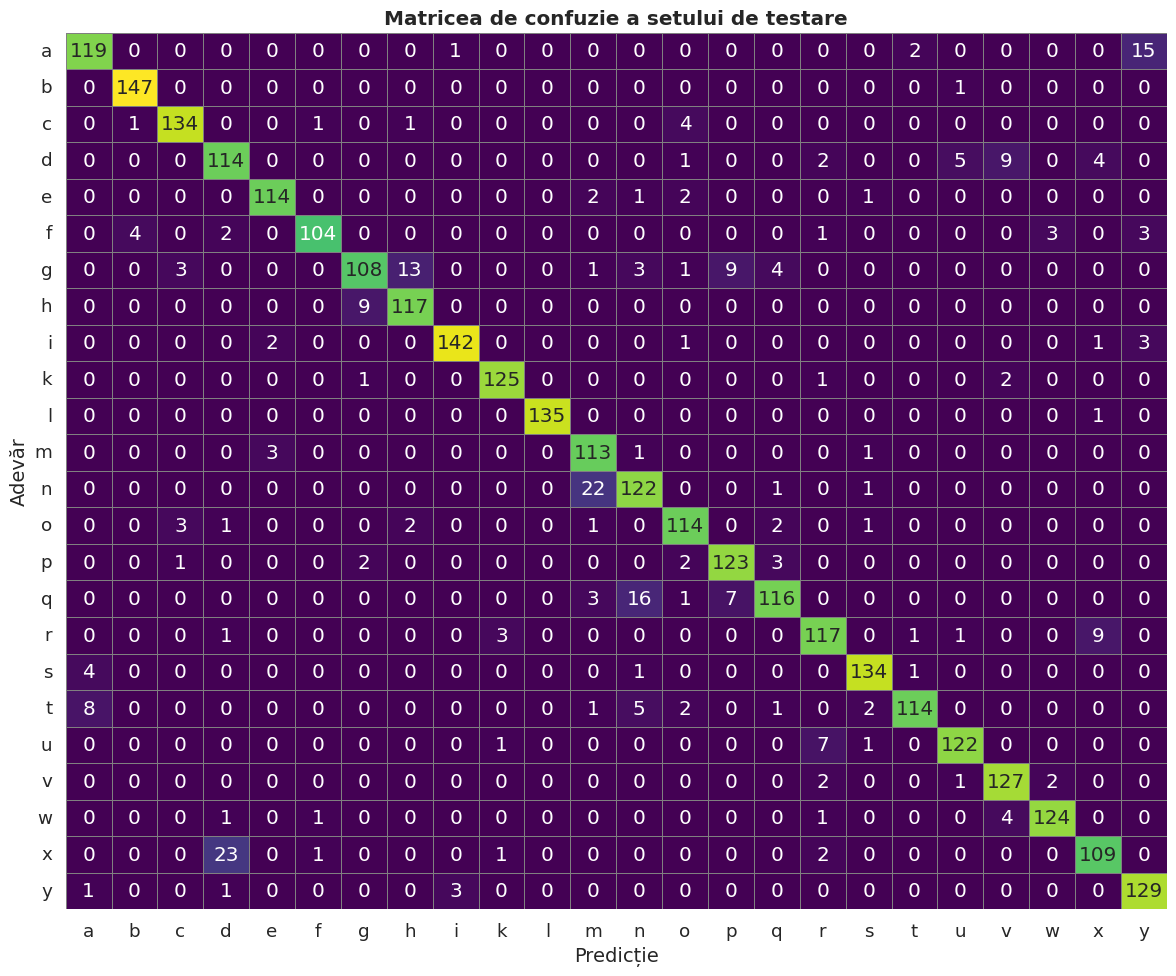
\includegraphics[width=0.55\textwidth]{images/2-recunoasterea-asl/conf_matrix_test_set.png}
  \caption[Matricea de confuzie a setului de testare]{\textbf{Matricea de confuzie a setului de testare}. \textit{Ilustrăm matricea de confuzie cu ajutorul unei hărți termice. Diagonala principală reprezintă numărul de exemple prezise corect pentru fiecare literă.}}
  \label{fig:conf_matrix_test_set}
\end{figure}

Mai departe, în Figura~\ref{fig:acc_per_class} poate fi analizată acuratețea pentru fiecare literă. Literele cele mai ușor de recunoscut de către modelul creat sunt B și L, cu acuratețe de $99,3\%$, iar cele care ridică probleme sunt G, cu o acuratețe de $76,1\%$, și X, cu acuratețe de $80,1\%$.

\begin{figure}[H]
  \centering
  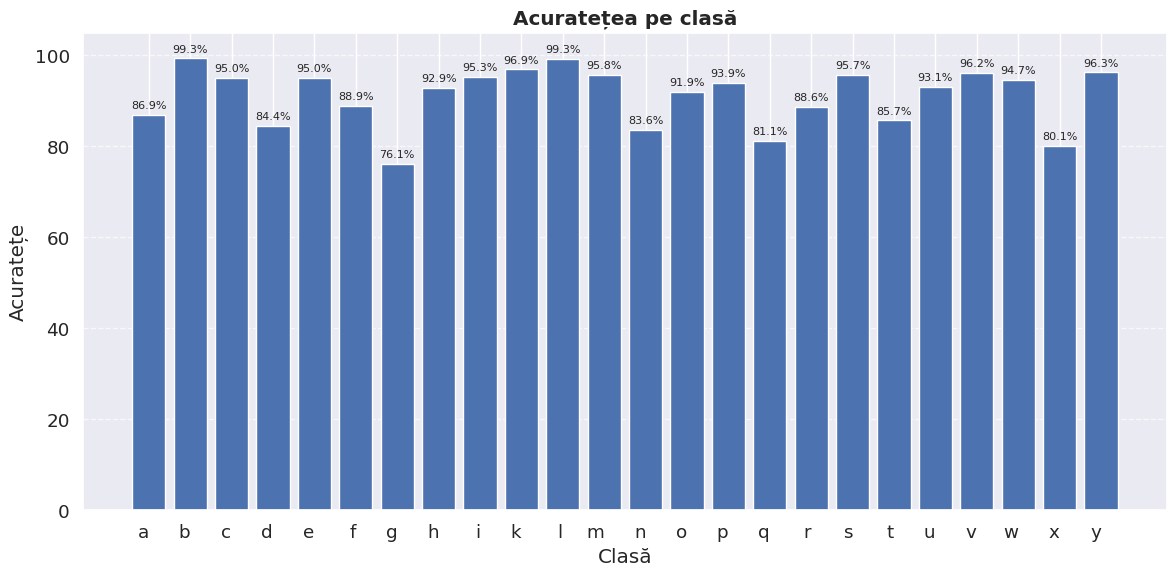
\includegraphics[width=0.7\textwidth]{images/2-recunoasterea-asl/acc_per_class.png}
  \caption[Acuratețea pe clasă]{\textbf{Acuratețea pe clasă}. \textit{Ilustrăm acuratețea predicțiilor pentru fiecare literă. Acuratețea este notată în vârful dreptunghiurilor reprezentative pentru clasa respectivă.}}
  \label{fig:acc_per_class}
\end{figure}

În final, am creat un raport de clasificare. În Tabela~\ref{tab:classif_report} putem observa cum litera G are un scor \textit{recall} scăzut (0.76), ceea ce înseamnă că există dificultăți în a recunoaște acea clasă. Combinând acest fapt cu datele din matricea de confuzie, putem concluziona că de multe ori, modelul are tendința să confunde G cu H, clasificând litera G ca fiind H. Mai mult de atât, chiar dacă litera Y are o acuratețe ridicată, poate fi observat cum scorul \textit{precision} este mai scăzut (0.86), sugerând faptul că modelul tinde să prezică Y și în situații în care aceasta nu este litera corectă.

\begin{table}[H]
\centering
\scriptsize
\begin{tabular}{c c c c c}
\toprule
\textbf{Clasă} & \textbf{Precizie} & \textbf{Recall} & \textbf{Scor F1} & \textbf{Număr exemple} \\
\midrule
a & 0.90 & 0.87 & 0.88 & 137 \\
b & 0.97 & 0.99 & 0.98 & 148 \\
c & 0.95 & 0.95 & 0.95 & 141 \\
d & 0.80 & 0.84 & 0.82 & 135 \\
e & 0.96 & 0.95 & 0.95 & 120 \\
f & 0.97 & 0.89 & 0.93 & 117 \\
g & 0.90 & 0.76 & 0.82 & 142 \\
h & 0.88 & 0.93 & 0.90 & 126 \\
i & 0.97 & 0.95 & 0.96 & 149 \\
k & 0.96 & 0.97 & 0.97 & 129 \\
l & 1.00 & 0.99 & 1.00 & 136 \\
m & 0.79 & 0.96 & 0.87 & 118 \\
n & 0.82 & 0.84 & 0.83 & 146 \\
o & 0.89 & 0.92 & 0.90 & 124 \\
p & 0.88 & 0.94 & 0.91 & 131 \\
q & 0.91 & 0.81 & 0.86 & 143 \\
r & 0.88 & 0.89 & 0.88 & 132 \\
s & 0.95 & 0.96 & 0.95 & 140 \\
t & 0.97 & 0.86 & 0.91 & 133 \\
u & 0.94 & 0.93 & 0.93 & 131 \\
v & 0.89 & 0.96 & 0.93 & 132 \\
w & 0.96 & 0.95 & 0.95 & 131 \\
x & 0.88 & 0.80 & 0.84 & 136 \\
y & 0.86 & 0.96 & 0.91 & 134 \\
\bottomrule
\end{tabular}
\caption[Raport de clasificare]{Pentru fiecare clasă, raportăm numărul de exemple testate și scorurile: precizie, recall și F1.}
\label{tab:classif_report}
\end{table}


\section{Evaluare experimentală}

Înainte de a avea arhitectura finală a rețelei neuronale convoluționale, au fost încercate diferite modele și tipuri de imagini.

În faza incipientă, imaginile au fost utilizate în forma lor originală, fără decuparea mâinii cu ajutorul MediaPipe Hands. Pentru a ne asigura că setul de date este corect, am antrenat un model cu arhitectura ResNet50 timp de 50 de epoci, obținând o acuratețe de $89.5\%$ pe setul de validare. După ce am confirmat corectitudinea setului de date, s-a optat pentru arhitecturi mai simple, deoarece ResNet50 are aproximativ 25M parametri, ceea ce este considerat ineficient pentru rularea locală pe dispozitive mobile.

Încercând cu arhitecturi proprii, am ajuns la acuratețe de aproximativ $68\%$, cu modele care au între 300.000 și 10.000.000 de parametri. Principalele dificultăți întâmpinate au fost reprezentate de subînvățare și supraînvățare. Pe lângă numărul de parametri, arhitectura a ridicat probleme și în funcție de așezarea straturilor convoluționale și rata creșterii numărului de canale. În cazul în care dublam numărul canalelor la fiecare strat convoluțional, de exemplu 3 \rightarrow\space 32 \rightarrow\space 64 \rightarrow\space 128 \rightarrow\space 256 \rightarrow\space 512, modelul devenea rapid prea complex și evaluarea începea să indice memorarea setului de date.

Printre algoritmii de ajustare a ratei de învățare, se numără \textit{ReduceLROnPlateau}, care reduce $\eta$ când învățarea stagnează, și \textit{CosineAnnealingWarmRestarts}, care resetează $\eta$ la un anumit punct, readucând rata de învățare la valoarea inițială, pentru a scăpa din minime locale și a încerca alte „drumuri” către convergență. În ambele cazuri, rezultatele nu erau cele așteptate, cele mai bune rezultate fiind observate prin utilizarea algoritmului CosineAnnealing.

Un punct de cotitură în cadrul testelor noastre a fost atins când am hotărât să utilizăm MediaPipe Hands pentru a extrage cadre cu mâinile. Acuratețea a început să crească considerabil, atingând deseori $90\%$, cu arhitecturi care conțineau aproximativ 1.000.000 de parametri. 

Pe lângă modelul prezentat în Capitolul~\ref{cap:cap2}, am antrenat și un MobileNetV3Large \cite{mobilenetv3}, care a atins acuratețe de $95,96\%$ pe setul de validare. Scopul acestui model era de a-l introduce ca opțiune de utilizare în aplicație pentru dispozitive performante, însă după convertirea într-un format compatibil cu Android, timpul de detecție pe cadru creștea considerabil și nu am putut identifica cauza precisă.

În ceea ce privește augmentarea datelor, trebuie menționat că, în cazul CutMix și Mixup, etichetele trebuie reprezentate ca vectori soft, conform articolului original dedicat metodei CutMix. Autorii menționează că utilizarea doar a etichetei dominante oferă rezultate mai bune decât absența aceastei metode de augmentare, însă rezultatele cele mai bune vor fi obținute prin utilizarea etichetelor soft. În urma experimentelor noastre, am observat că prin utilizarea etichetelor soft, a arhitecturii dezvoltate și a hiperparametrilor prezentați în această lucrare, acuratețea maximă obținută a fost de doar $89,15\%$.
\chapter{Aplicația mobilă și infrastructura aplicației}
\label{cap:cap3}

\section{Aplicația Android}
Aplicația Android servește drept mediu de interacțiune cu modelul discutat în capitolul anterior. Aceasta este scrisă cu ajutorul limbajului \textbf{Kotlin} \cite{kotlin}, utilizând biblioteca de instrumente pentru dezvoltare, \textbf{Jetpack Compose} \cite{jetpackcompose}. Detecțiile au loc la nivel local, modelul fiind încărcat pe dispozitivul Android cu ajutorul \textbf{PyTorch Mobile}. Interfața pentru cameră este oferită de biblioteca \textbf{CameraX} \cite{camerax}, iar cererile \textit{HTTP}, transmise prin protocolul securizat \textit{HTTPS}, sunt facilitate de biblioteca \textbf{Retrofit} \cite{retrofit}. Ecranele prezentate în acest capitol funcționează pe baza unei stive gestionate cu ajutorul unui obiect de tip \textit{NavController}. În continuare, detaliem structura și fluxul logic al aplicației.

\textbf{Ecranul de bun-venit}. După deschiderea aplicației, utilizatorul este întâmpinat de ecranul de bun-venit (Figura~\ref{fig:welcome_screen}), unde îi sunt prezentate trei opțiuni: \textit{Sign In} (autentificare), \textit{Sign Up} (crearea unui cont nou) sau \textit{Skip and use offline} (simpla detectare a literelor). Aplicația afișează acest meniu doar în cazurile în care utilizatorul nu este autentificat sau este autentificat, dar dispozitivul nu este conectat la internet.


\textbf{Utilizarea fără conexiune la internet}. Această opțiune oferă  posibilitatea de a detecta literele fără autentificare, pentru a asigura o experiență cât mai plăcută și accesibilă utilizatorilor care își doresc să acceseze doar funcția de traducere. Aplicația încarcă modelul în memorie și încearcă să detecteze mâini afișate pe ecran cu ajutorul algoritmului MediaPipe Hands. Odată ce o mână este detectată, este decupat un dreptunghi care încadrează mâna și transmis mai departe către modelul responsabil pentru detecția literei. În cazul în care este detectat un semn valid, este afișată litera recunoscută (Figura~\ref{fig:offline_valid_detection}), iar în caz contrar, este afișat caracterul „-” (Figura~\ref{fig:offline_invalid_detection}).


\begin{figure}[H]
  \centering
  \begin{subfigure}{0.2\textwidth}
    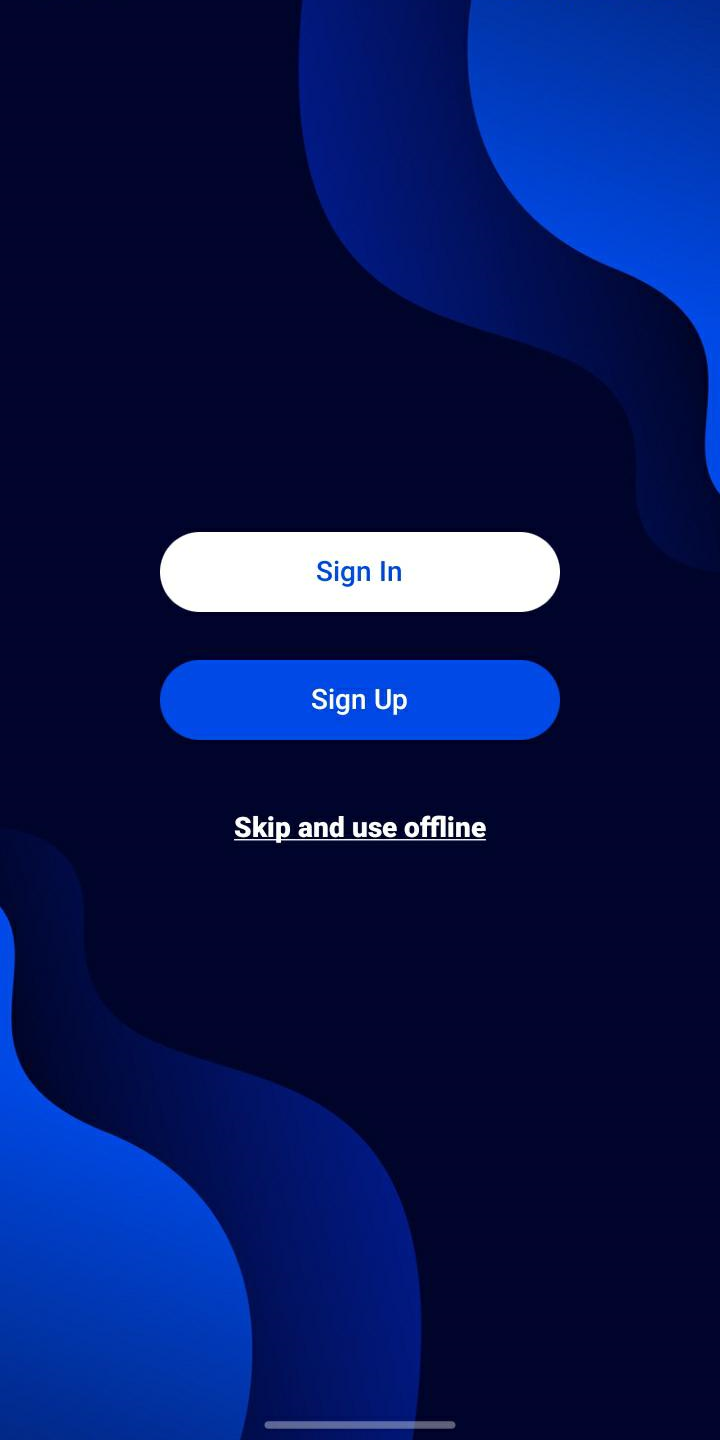
\includegraphics[width=\linewidth]{images/3-aplicatia-android/welcome_screen_android_app.png}
    \caption{}
    \label{fig:welcome_screen}
  \end{subfigure}
  \begin{subfigure}{0.2\textwidth}
    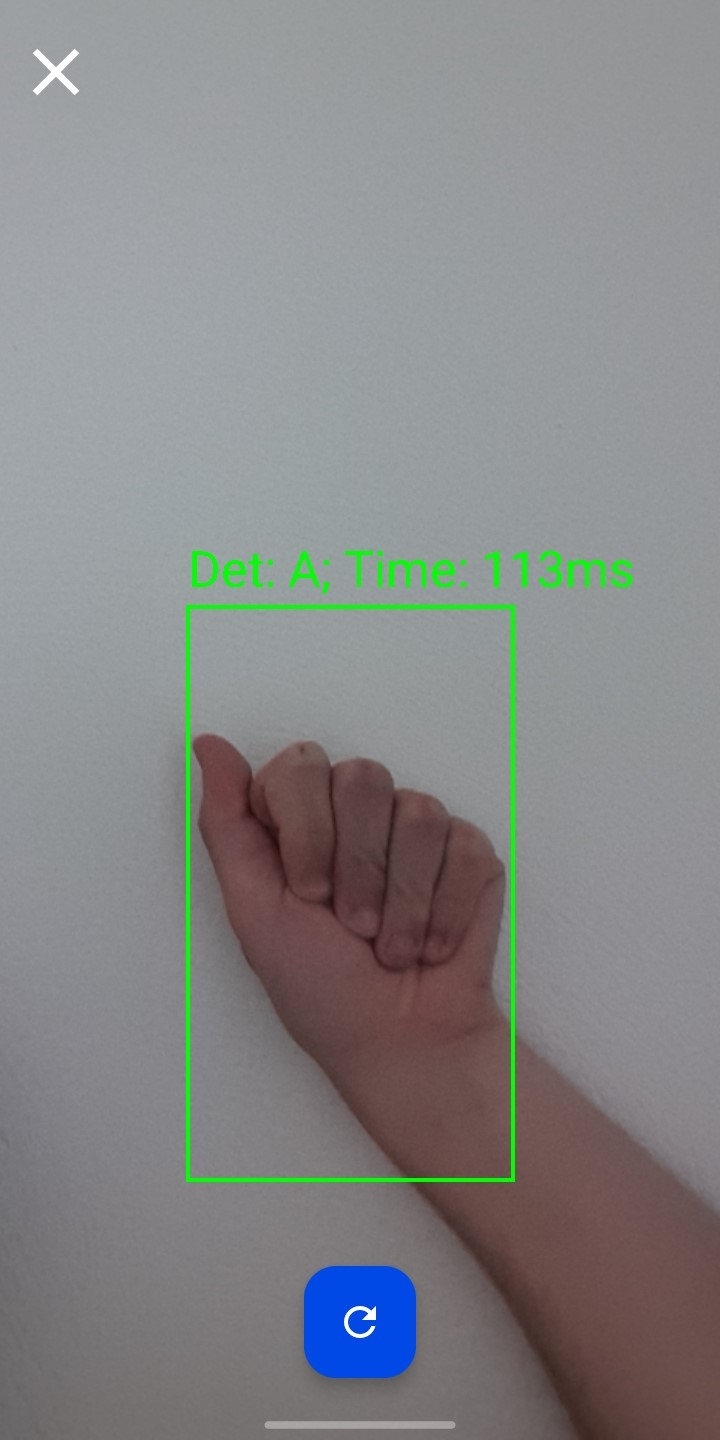
\includegraphics[width=\linewidth]{images/3-aplicatia-android/ffa_detection.jpeg}
    \caption{}
    \label{fig:offline_valid_detection}
  \end{subfigure}
  \begin{subfigure}{0.2\textwidth}
    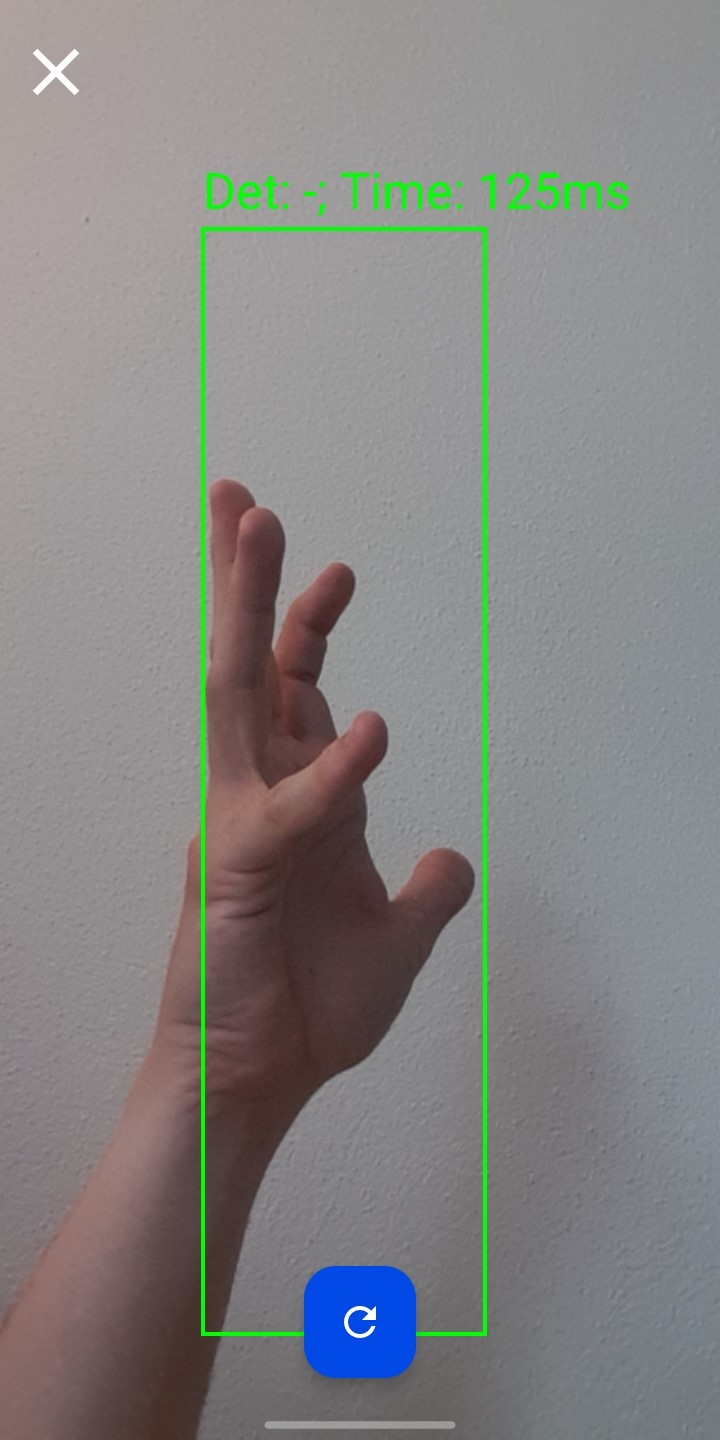
\includegraphics[width=\linewidth]{images/3-aplicatia-android/ffa_invalid_detection.jpeg}
    \caption{}
    \label{fig:offline_invalid_detection}
  \end{subfigure}
  \caption[Ecranele inițiale ale aplicației]{\textbf{Ecranele inițiale ale aplicației}. \textit{Ilustrăm ecranele inițiale ale aplicației. (a) ilustrează ecranul de bun-venit, unde sunt prezente butoanele de Sign In, Sign Up și Skip and use offline; (b) ilustrează modul de detecție în lipsa conexiunii la internet; palma detectată de MediaPipe Hands este încadrată în chenarul verde, deasupra căruia utilizatorul este înștiințat ca a fost detectată litera A, într-un timp de 113ms; (c) ilustrează momentul în care utilizatorul afișează un semn invalid.}}
  \label{fig:welcome_screen_offline_det_screen}
\end{figure}

\textbf{Autentificarea utilizatorilor}. Utilizatorul are posibilitatea de a crea un cont nou, de a se conecta cu datele sale, de a schimba parola și de a se deconecta.

Pentru început, utilizatorul apasă butonul de Sign Up, pentru a introduce adresa de email și parola noului cont (Figura~\ref{fig:sign_up_screen}). După o validare a câmpurilor, aplicația trimite datele către server. În cazul în care serverul oferă un răspuns pozitiv, utilizatorului îi este afișat ecranul de validare a adresei de email (Figura~\ref{fig:validation_screen}). În acest pas, utilizatorul află că are timp 5 minute pentru a introduce un cod primit pe email cu scopul de a confirma adresa. În urma unui răspuns valid din partea serverului privind codul de validare introdus, utilizatorul este înștiințat și redirecționat către ecranul de start, de unde se poate conecta cu noul său cont.


În urma apăsării butonului de Sign In, este afișat un ecran care oferă posibilitatea de a introduce datele contului (Figura~\ref{fig:sign_in_screen}), care sunt transmise către server pentru validare. În cazul unui răspuns pozitiv, utilizatorul este direcționat către meniul principal, unde poate opta pentru începerea unei sesiuni de antrenament în învățarea alfabetului ASL. Mai mult decât atât, odată cu răspunsul pozitiv, dispozitivul primește un \textbf{JSON Web Token} (JWT) \cite{jwt}, denumit token de acces, alături de un token de reîmprospătare. Detalii despre această metodă sunt oferite în Secțiunea~\ref{sec:server_app}.


În cazul în care utilizatorul își uită parola, acesta poate face o cerere de schimbare a parolei, care constă în introducerea adresei de email către care sunt trimise instrucțiunile pentru resetare (Figura~\ref{fig:forgot_password}).

\begin{figure}[H]
  \centering
  \begin{subfigure}{0.2\textwidth}
    \includegraphics[width=\linewidth]{images/3-aplicatia-android/sign_up_screen.jpeg}
    \caption{}
    \label{fig:sign_up_screen}
  \end{subfigure}
  \begin{subfigure}{0.2\textwidth}
    \includegraphics[width=\linewidth]{images/3-aplicatia-android/validation_code_screen.jpeg}
    \caption{}
    \label{fig:validation_screen}
  \end{subfigure}
  \caption[Crearea unui cont nou]{\textbf{Crearea unui cont nou}. \textit{Ilustrăm procesul de creare a unui cont nou. (a) ilustrează cele trei câmpuri necesare creării unui nou cont: email, parola, confirmarea parolei; (b) ilustrează înștiințarea utilizatorului de timpul rămas pentru introducerea codului de validare primit pe email, printr-un temporizator; în fiecare câmp trebuie introdusă câte o cifră.}}
  \label{fig:sign_up_validation_screens}
\end{figure}


\begin{figure}[H]
  \centering
  \begin{subfigure}{0.2\textwidth}
    \includegraphics[width=\textwidth]{images/3-aplicatia-android/sign_in_screen.jpeg}
  \caption{}
  \label{fig:sign_in_screen}
  \end{subfigure}
  \begin{subfigure}{0.2\textwidth}
    \includegraphics[width=\linewidth]{images/3-aplicatia-android/forgot_pass_screen.jpeg}
    \caption{}
    \label{fig:forgot_password}
  \end{subfigure}
  \caption[Conectare și resetarea parolei]{\textbf{Conectare și resetarea parolei}. \textit{(a) ilustrează câmpurile necesare pentru conectare (email și parolă), alături de butoanele Sign In pentru conectare și Forgot Password pentru resetarea parolei; (b) ilustrează ecranul pentru crearea unei cereri de restare a parolei.}}
  \label{fig:sign_up_validation_screens}
\end{figure}

\textbf{Meniul principal}. Meniul prezentat în Figura~\ref{fig:main_menu_screen} îi permite utilizatorului să aleagă între a învăța alfabetul ASL și a se deconecta. Deconectarea trimite o cerere către server pentru a invalida sesiunea și șterge token-urile prezente pe dispozitiv. Dacă utilizatorul apasă butonul \textit{Start learning}, camera se deschide și este inițiată o nouă sesiune de antrenament.

\textbf{Sesiune de învățare a alfabetului ASL}. Odată cu începerea unei sesiuni de antrenament, utilizatorul primește înștiințarea că este necesară introducerea mâinii în cadru (Figura~\ref{fig:start_learn_prompt}). Pe urmă, este afișată prima literă din alfabet, care rămâne pe ecran cât timp modelul nu recunoaște corect litera indicată (Figura~\ref{fig:learning_started}). Odată ce litera afișată este detectată, sesiunea continuă automat la următoarea literă din alfabet (Figura~\ref{fig:first_letter_detected}).

\begin{figure}[H]
\centering
    \includegraphics[width=0.2\textwidth]{images/3-aplicatia-android/main_menu_screen.jpeg}
  \caption[Meniul principal]{\textbf{Meniul principal}. \textit{Ilustrăm meniul principal care oferă opțiunile de începere a unei sesiuni de antrenament (Start Learning) și de decontectare (Log Out).}}
  \label{fig:main_menu_screen}
\end{figure}

\begin{figure}[H]
  \centering
    \begin{subfigure}{0.2\textwidth}
    \includegraphics[width=\textwidth]{images/3-aplicatia-android/start_learn_screen.jpeg}
  \caption{}
  \label{fig:start_learn_prompt}
  \end{subfigure}
 \begin{subfigure}{0.2\textwidth}
    \includegraphics[width=\textwidth]{images/3-aplicatia-android/learning_started.jpeg}
  \caption{}
  \label{fig:learning_started}
  \end{subfigure}
   \begin{subfigure}{0.2\textwidth}
    \includegraphics[width=\textwidth]{images/3-aplicatia-android/learn_a_detected.jpeg}
  \caption{}
  \label{fig:first_letter_detected}
  \end{subfigure}
  \caption[Sesiune de învățare]{\textbf{Sesiune de învățare}. \textit{(a) ilustrează instrucțiunea primită de utilizator pentru a își introduce palma în cadru; (b) ilustrează începerea sesiunii de învățare prin afișarea literei A; (c) ilustrează afișarea literei B. Utilizatorul află ce literă învață prin afișarea caracterului cu culoarea verde, iar dedesubt se află o imagine care ilustrează semnul pentru acea literă.}}
  \label{fig:training_sesh_figs}
\end{figure}

\section{Infrastructura aplicației}
\label{sec:server_app}
Arhitectura aplicației urmează o structură containerizată folosind \textbf{Docker} \cite{docker}, prin \textit{docker-compose}, ceea ce oferă un mediu de execuție portabil și izolat. Aplicația are la bază 4 containere:

\begin{itemize}
    \item \textbf{Uvicorn} + \textbf{FastAPI} - server asincron \cite{uvicorn} care răspunde cererilor HTTP prin cadrul de dezvoltare \textbf{FastAPI} \cite{fastapi}, care gestionează logica aplicației și oferă suport în gestionarea măsurilor de securitate.
    \item \textbf{PostgreSQL} - bază de date relațională, care asigură stocarea persistentă a datelor \cite{postgresql}.
    \item \textbf{Redis} - bază de date în memorie care funcționează pe bază de cheie-valoare \cite{redis} și asigură accesul rapid asupra datelor.
    \item \textbf{NGINX} - reverse proxy \cite{nginx} care preia cererile HTTP și le redirecționează către serverul Uvicorn, gestionează traficul și asigură conexiuni securizate prin \textit{SSL}.
\end{itemize}

\textbf{Server}. Serverul are la bază o arhitectură orientată pe servicii (SOA), structurată în straturi decuplate în funcție de responsabilitate. O cerere HTTP parcurge un flux logic de tipul: \textbf{API} \rightarrow \space\textbf{serviciu} (logica aplicației) \rightarrow\space \textbf{CRUD} (acces la baza de date) \rightarrow\space răspuns.

Conexiunea către baza de date este creată utilizând componenta de acces la baza de date în mod asincron oferită de biblioteca \textbf{asyncpg} \cite{asyncpg}, iar relația dintre entitățile bazei de date și modelele relaționale definite în cod este facilitată de biblioteca \textbf{SQLModel} \cite{sqlmodel}.

Relația de dependență dintre servicii este facilitată de clasa \textit{Depends} din biblioteca FastAPI, care asigură mecanismul de injectare a dependențelor. De exemplu, clasa \textit{AuthService} este injectată în \textit{endpoint}-urile pentru autentificare, iar clasele \textit{UserService} și \textit{RedisClient} sunt injectate în clasa AuthService, aceasta din urmă depinzând de cele două.

Pe lângă înregistrarea de conturi noi și capacitatea de a conecta și deconecta utilizatori de la aplicație, serverul are ca funcționalități și schimbarea parolelor și reîmprospătarea token-urilor de acces.

Pentru procesarea unei cererei de înregistrare, este validată adresa de email  cu ajutorul bibliotecii \textbf{email-validator} \cite{email_validator}. În urma validării, se verifică lipsa adresei în baza de date și a potrivirii textelor introduse în cele două câmpuri desemnate parolei. În continuare, se aplică o funcție de dispersie (în engl. \textit{hash}) asupra parolei cu ajutorul bibliotecii \textbf{bcrypt} \cite{bcrypt}, iar datele utilizatorului sunt salvate. În final, este generat un cod unic de verificare care este trimis printr-un email către utilizator, cu scopul de a verifica adresa de email. Adresa și codul de verificare sunt salvate ca pereche cheie-valoare, unde codul reprezintă cheia și emailul reprezintă valoarea, într-o bază de date Redis, cu timp de expirare de cinci minute. Utilizatorul nu poate folosi datele sale de acces până nu confirmă adresa de email.


În urma validării contului de email, utilizatorul se poate conecta la noul său cont, moment în care sunt verificate datele sale de autentificare. Alături de un răspuns pozitiv, serverul trimite și un obiect de tip \textit{AuthorizationTokens}, care conține un token de acces și un token de reîmprospătare.

Pentru deconectare, clientul trimite către server token-ul de acces salvat pe dispozitiv și token-ul de reîmprospătare asociat. În cazul validării token-ului de acces, token-ul de reîmprospătare este invalidat, iar utilizatorul este deconectat și redirecționat către ecranul de bun-venit.



\textbf{Token de acces și token de reîmprospătare}. Timpul de expirare a token-ului de acces este, în cazul nostru, de o oră, și este semnat cu o cheie secretă, pentru a ne asigura, la recepționare, că acesta nu a fost manipulat în vreun fel. Avantajele JWT provin din principiul lipsei de stare pe care îl respectă, acesta nefiind stocat pe serverul aplicației, ci doar pe dispozitivul utilizatorului.

Rolul token-ului de reîmprospătare este vizibil în momentul în care expiră JWT. Acesta este stocat în baza de date Redis și este folosit pentru crearea unui nou JWT. Tandemul token de acces - token de reîmprospătare oferă utilizatorului o experiență plăcută în navigarea prin aplicație, deoarece toate verificările sunt făcute în fundal, fără a fi necesare reconectări manuale frecvente. Token-ul de reîmprospătare este valabil, în cazul nostru, timp de 30 de zile, perioadă la finalul căreia utilizatorul trebuie să se conecteze din nou.

\textbf{Persistența datelor}. Stocarea datelor este facilitată de o bază de date relațională de tip PostgreSQL și de o bază de date în memorie, Redis.

Baza de date relațională este folosită pentru a salva datele utilizatorilor și conține o tabelă numită \textit{users}. Coloana \textit{id} este cheia primară, de tip \textit{UUID4}, \textit{email} și \textit{password} sunt de tip \textit{VARCHAR}, iar \textit{confirmed} este de tip \textit{boolean} și asigură confirmarea contului.


Pentru a avea o experiență fluentă în utilizarea aplicației, am optat pentru stocarea token-urilor de reîmprospătare și a codurilor de acces într-o bază de date Redis. Token-urile de reîmprospătare, codurile de validare a adreselor de email și cele pentru schimbarea parolelor sunt accesate cu un timp de latență minim. Toate cheile sunt salvate după ce au fost schimbate de o funcție hash, pentru a spori securitatea.

\textbf{Reverse proxy}. Toate cererile ajung mai întâi la containerul pentru NGINX, care le filtrează în funcție de cerințele notate în fișierul pentru configurări. În primul rând, sunt acceptate doar cereri HTTPS, containerul utilizând un certificat SSL. NGINX primește cereri la adresa \url{https://localhost:443}. De asemenea, am implementat un mecanism de limitare a numărului de cereri din partea unui singur utilizator, pentru a descuraja trimiterea unui număr ridicat de cereri într-un interval scurt. În urma filtrării, acestea sunt redirecționate către \url{http://uv-app:8000}, unde \textit{uv-app} este numele containerului care rulează serverul Uvicorn.
\chapter{Direcții viitoare și concluzii}
\label{cap:cap4}

\section{Direcții viitoare}

A fost dificil de atins un echilibru optim între subînvățare și supraînvățare. Performanța maximă a modelului prezentat în lucrare, cu o acuratețe de $92,45\%$ pe setul de antrenare, sugerează că există în continuare potențial pentru îmbunătățiri. O posibilă cauză a stagnării ar putea fi regularizarea excesivă, utilizând augmentare puternică a datelor, dropout, label smoothing și weight decay. 

Privind modelul MobileNetV3Large, este necesară o investigație amănunțită pentru a detecta cauza scăderii semnificative a eficienței modelului în urma conversiei în format compatibil cu Android. Se pot lua în considerare utilizarea altor instrumente sau metode de conversie.

Referitor la setul de date, acesta ar putea avea imagini incorecte, întrucât imaginile au fost filtrate manual, acțiune predispusă la eroarea umană. În plus, anumite litere au exemple din multiple dialecte, ceea ce ar putea induce în eroare modelul. O metodă de a combate acest lucru este păstrarea unui singur dialect pentru fiecare literă și antrenarea folosind ponderi pentru clase, astfel încât clasele subreprezentate să poată avea o pondere mai mare decât cele cu un număr mai ridicat de exemple.

Aplicația Android poate avea mai multe funcționalități, în special pentru utilizatorii conectați. Aceștia ar putea avea sesiunile de învățare salvate, cu posibilitatea de a le analiza și observa o evoluție a progresului. De asemenea, poate fi introdusă o secțiune cu sesiuni de antrenament specializate, cu literele la care utilizatorul prezintă probleme. Corectitudinea sesiunii de antrenament ar putea fi bazată pe siguranța modelului. Cu cât predicția este mai sigură, cu atât litera a fost mai aproape de realitate, iar bazat pe siguranța aceasta, utilizatorul ar putea primi sugestiile menționate anterior.

\section{Concluzii}
Lucrarea de licență prezentată a avut ca scop reducerea dificultăților de comunicare dintre persoanele cu deficiențe de auz și/sau vorbire și populația generală. Soluția propusă constă într-o aplicație mobilă, creată pentru sistemul de operare Android și are la bază o rețea neuronală convoluțională. 

Centrul acestei aplicații este un model CNN utilizat în recunoașterea alfabetului limbajului semnelor american. Considerăm că, prin crearea unui set de date propriu, obținut prin combinarea mai multor surse, am adus o contribuție literaturii de specialitate și domeniului experimental datorită diversității imaginilor. Arhitectura propusă este una eficientă și combină elemente simple și de bază din domeniile vederii artificiale și învățării automate supervizate. Modelul atinge o acuratețe de $91,06\%$ pe setul de testare, care conține imagini reprezentative pentru lumea reală. Pe un dispozitiv \textbf{Samsung Galaxy S9}, timpul de inferență este de aproximativ 120ms, timp care include și extragerea palmei prin MediaPipe Hands (12ms), așa că poate fi utilizat în timp real, fără întârzieri evidente majore.

În concluzie, lucrarea și-a atins obiectivul de a dezvolta o aplicație funcțională pentru traducerea alfabetului ASL, care totodată reprezintă și un punct de plecare pentru o aplicație avansată, capabilă să traducă cuvinte și propoziții.
\printbibliography[heading=bibintoc]
\end{document}